% Created by tikzDevice version 0.12.6 on 2024-05-22 14:37:09
% !TEX encoding = UTF-8 Unicode
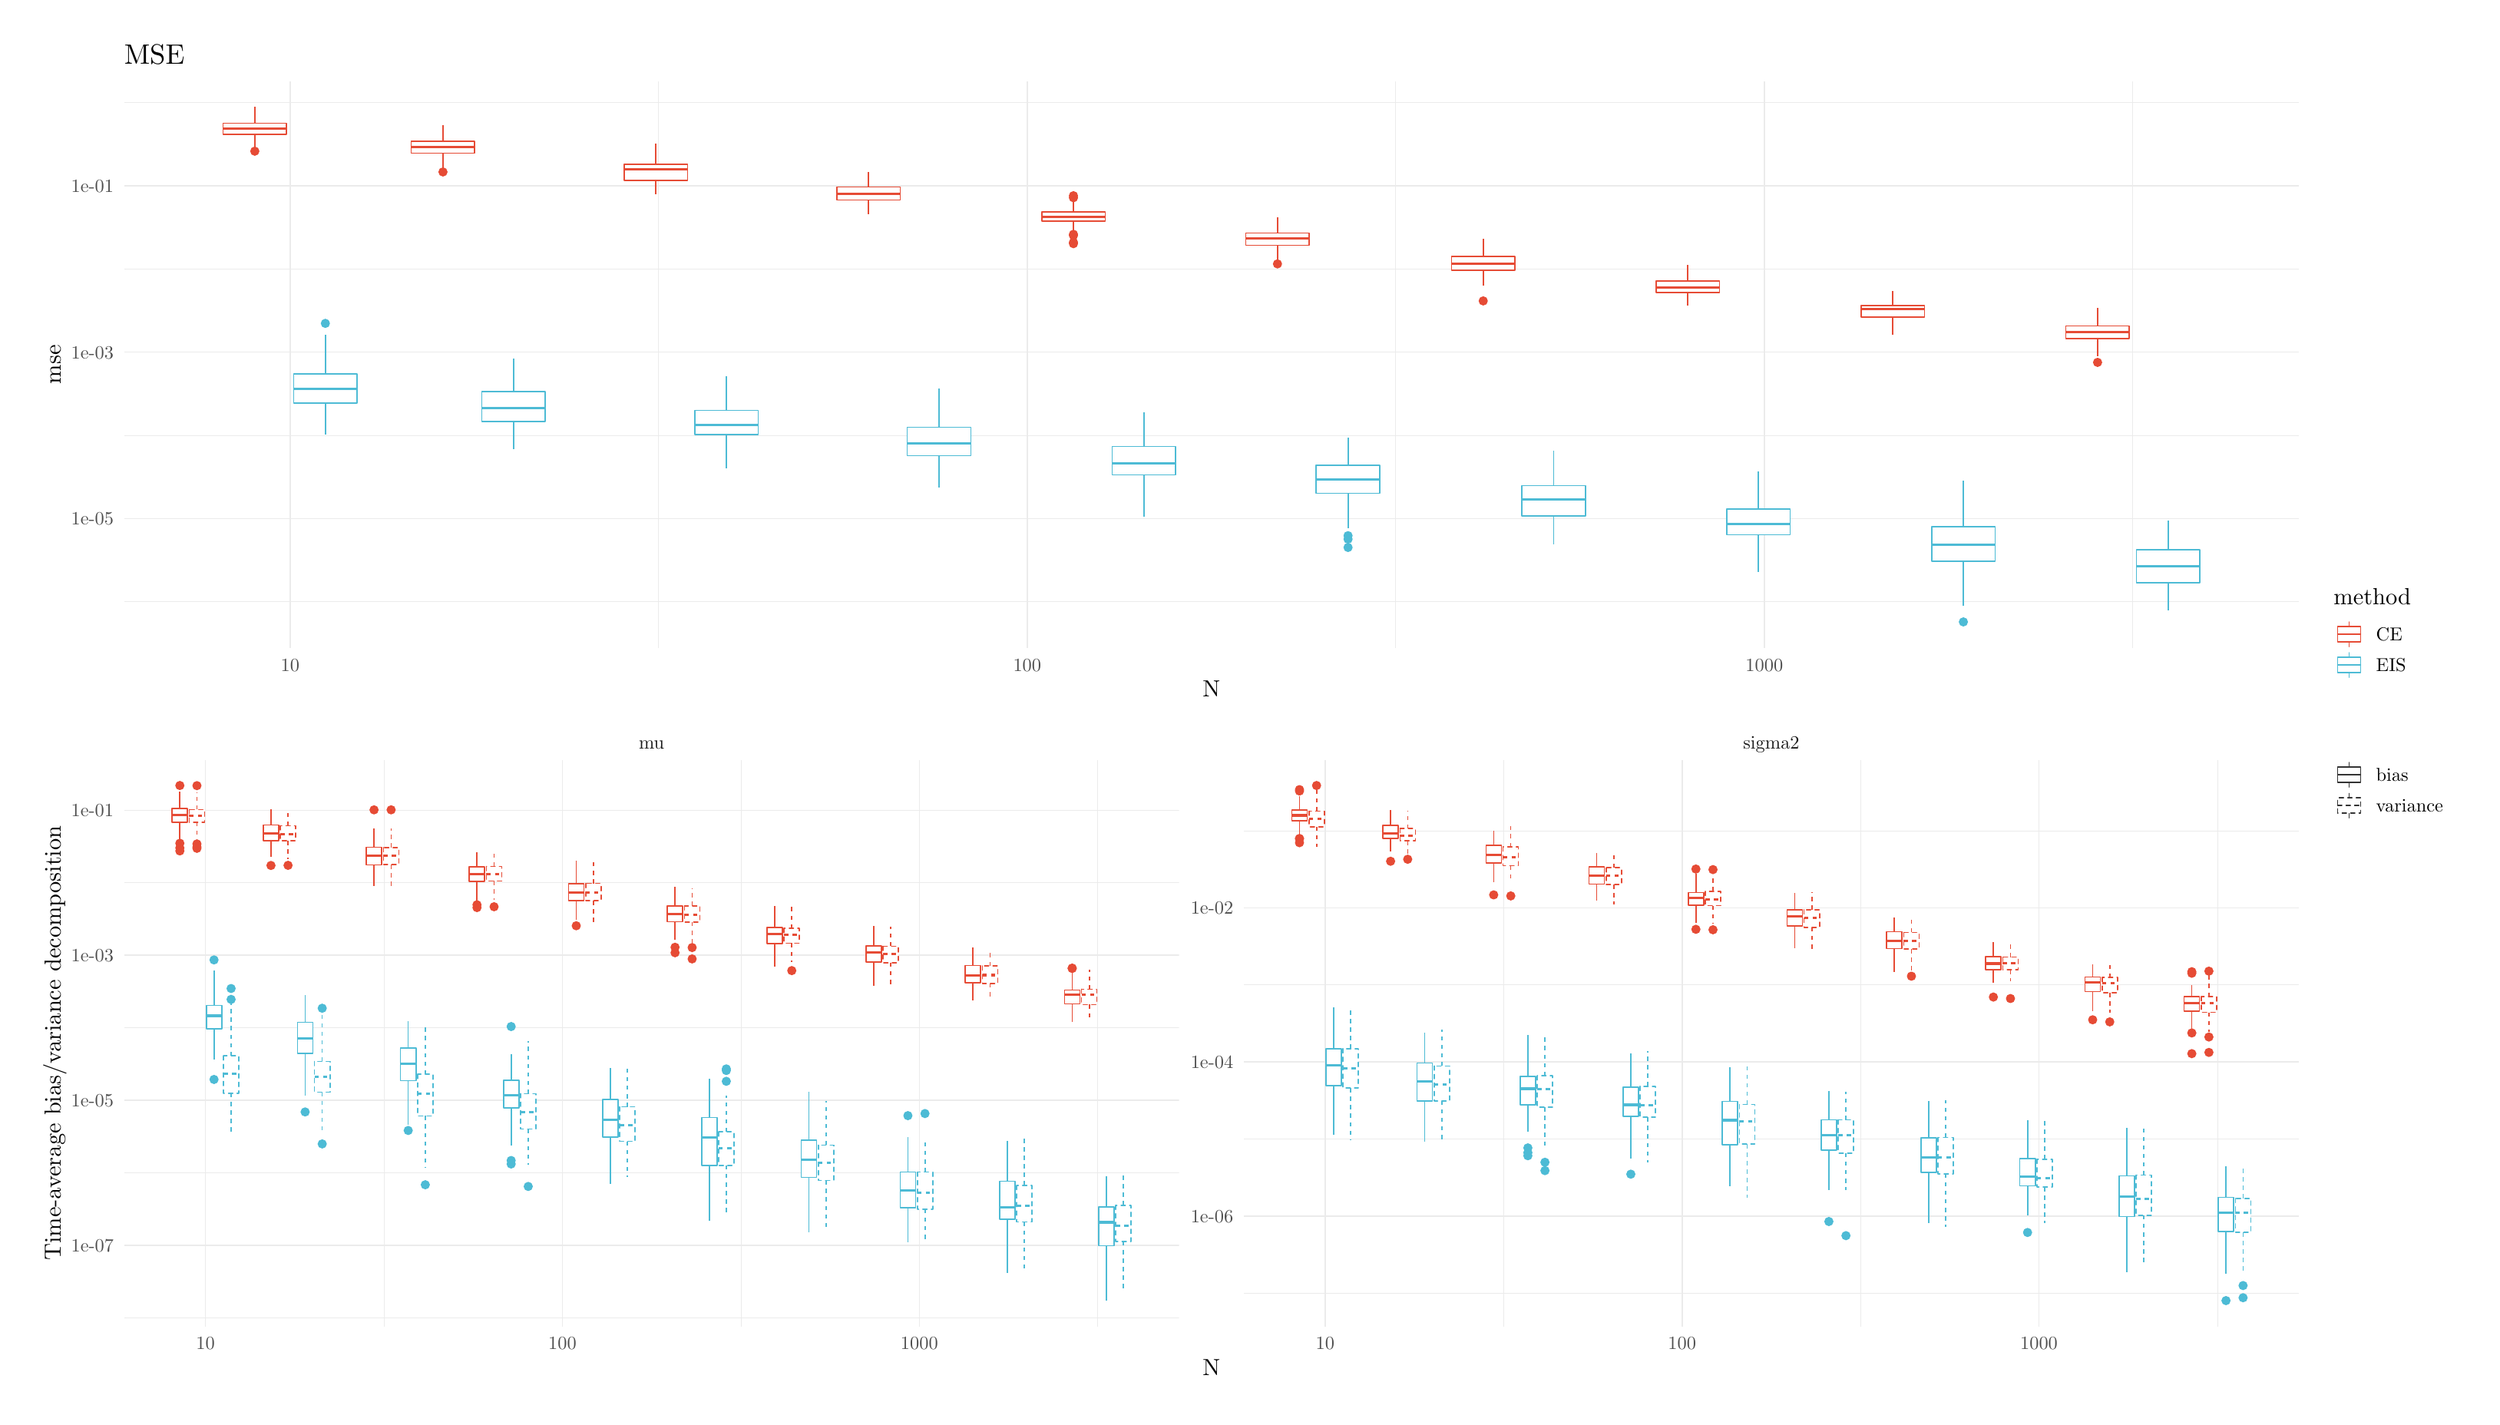
\begin{tikzpicture}[x=1pt,y=1pt]
\definecolor{fillColor}{RGB}{255,255,255}
\path[use as bounding box,fill=fillColor,fill opacity=0.00] (0,0) rectangle (1156.32,650.43);
\begin{scope}
\path[clip] ( 48.45,355.61) rectangle (1071.82,622.27);
\definecolor{drawColor}{gray}{0.92}

\path[draw=drawColor,line width= 0.3pt,line join=round] ( 48.45,377.19) --
	(1071.82,377.19);

\path[draw=drawColor,line width= 0.3pt,line join=round] ( 48.45,455.52) --
	(1071.82,455.52);

\path[draw=drawColor,line width= 0.3pt,line join=round] ( 48.45,533.86) --
	(1071.82,533.86);

\path[draw=drawColor,line width= 0.3pt,line join=round] ( 48.45,612.20) --
	(1071.82,612.20);

\path[draw=drawColor,line width= 0.3pt,line join=round] (299.97,355.61) --
	(299.97,622.27);

\path[draw=drawColor,line width= 0.3pt,line join=round] (646.87,355.61) --
	(646.87,622.27);

\path[draw=drawColor,line width= 0.3pt,line join=round] (993.77,355.61) --
	(993.77,622.27);

\path[draw=drawColor,line width= 0.6pt,line join=round] ( 48.45,416.35) --
	(1071.82,416.35);

\path[draw=drawColor,line width= 0.6pt,line join=round] ( 48.45,494.69) --
	(1071.82,494.69);

\path[draw=drawColor,line width= 0.6pt,line join=round] ( 48.45,573.03) --
	(1071.82,573.03);

\path[draw=drawColor,line width= 0.6pt,line join=round] (126.52,355.61) --
	(126.52,622.27);

\path[draw=drawColor,line width= 0.6pt,line join=round] (473.42,355.61) --
	(473.42,622.27);

\path[draw=drawColor,line width= 0.6pt,line join=round] (820.32,355.61) --
	(820.32,622.27);
\definecolor{drawColor}{RGB}{230,75,53}
\definecolor{fillColor}{RGB}{230,75,53}

\path[draw=drawColor,line width= 0.4pt,line join=round,line cap=round,fill=fillColor] (109.91,589.27) circle (  1.96);

\path[draw=drawColor,line width= 0.6pt,line join=round] (109.91,602.43) -- (109.91,610.15);

\path[draw=drawColor,line width= 0.6pt,line join=round] (109.91,597.18) -- (109.91,589.35);
\definecolor{fillColor}{RGB}{255,255,255}

\path[draw=drawColor,line width= 0.6pt,line join=round,line cap=round,fill=fillColor] ( 94.97,602.43) --
	( 94.97,597.18) --
	(124.86,597.18) --
	(124.86,602.43) --
	( 94.97,602.43) --
	cycle;

\path[draw=drawColor,line width= 1.1pt,line join=round] ( 94.97,599.88) -- (124.86,599.88);
\definecolor{fillColor}{RGB}{230,75,53}

\path[draw=drawColor,line width= 0.4pt,line join=round,line cap=round,fill=fillColor] (198.47,579.50) circle (  1.96);

\path[draw=drawColor,line width= 0.6pt,line join=round] (198.47,594.01) -- (198.47,601.62);

\path[draw=drawColor,line width= 0.6pt,line join=round] (198.47,588.28) -- (198.47,581.12);
\definecolor{fillColor}{RGB}{255,255,255}

\path[draw=drawColor,line width= 0.6pt,line join=round,line cap=round,fill=fillColor] (183.52,594.01) --
	(183.52,588.28) --
	(213.41,588.28) --
	(213.41,594.01) --
	(183.52,594.01) --
	cycle;

\path[draw=drawColor,line width= 1.1pt,line join=round] (183.52,591.17) -- (213.41,591.17);

\path[draw=drawColor,line width= 0.6pt,line join=round] (298.65,583.04) -- (298.65,592.79);

\path[draw=drawColor,line width= 0.6pt,line join=round] (298.65,575.51) -- (298.65,568.86);

\path[draw=drawColor,line width= 0.6pt,line join=round,line cap=round,fill=fillColor] (283.71,583.04) --
	(283.71,575.51) --
	(313.59,575.51) --
	(313.59,583.04) --
	(283.71,583.04) --
	cycle;

\path[draw=drawColor,line width= 1.1pt,line join=round] (283.71,580.63) -- (313.59,580.63);

\path[draw=drawColor,line width= 0.6pt,line join=round] (398.71,572.42) -- (398.71,579.51);

\path[draw=drawColor,line width= 0.6pt,line join=round] (398.71,566.26) -- (398.71,559.75);

\path[draw=drawColor,line width= 0.6pt,line join=round,line cap=round,fill=fillColor] (383.77,572.42) --
	(383.77,566.26) --
	(413.65,566.26) --
	(413.65,572.42) --
	(383.77,572.42) --
	cycle;

\path[draw=drawColor,line width= 1.1pt,line join=round] (383.77,569.10) -- (413.65,569.10);
\definecolor{fillColor}{RGB}{230,75,53}

\path[draw=drawColor,line width= 0.4pt,line join=round,line cap=round,fill=fillColor] (495.18,549.62) circle (  1.96);

\path[draw=drawColor,line width= 0.4pt,line join=round,line cap=round,fill=fillColor] (495.18,568.31) circle (  1.96);

\path[draw=drawColor,line width= 0.4pt,line join=round,line cap=round,fill=fillColor] (495.18,567.37) circle (  1.96);

\path[draw=drawColor,line width= 0.4pt,line join=round,line cap=round,fill=fillColor] (495.18,550.15) circle (  1.96);

\path[draw=drawColor,line width= 0.4pt,line join=round,line cap=round,fill=fillColor] (495.18,546.37) circle (  1.96);

\path[draw=drawColor,line width= 0.4pt,line join=round,line cap=round,fill=fillColor] (495.18,545.75) circle (  1.96);

\path[draw=drawColor,line width= 0.6pt,line join=round] (495.18,560.64) -- (495.18,566.67);

\path[draw=drawColor,line width= 0.6pt,line join=round] (495.18,556.47) -- (495.18,551.07);
\definecolor{fillColor}{RGB}{255,255,255}

\path[draw=drawColor,line width= 0.6pt,line join=round,line cap=round,fill=fillColor] (480.23,560.64) --
	(480.23,556.47) --
	(510.12,556.47) --
	(510.12,560.64) --
	(480.23,560.64) --
	cycle;

\path[draw=drawColor,line width= 1.1pt,line join=round] (480.23,558.41) -- (510.12,558.41);
\definecolor{fillColor}{RGB}{230,75,53}

\path[draw=drawColor,line width= 0.4pt,line join=round,line cap=round,fill=fillColor] (591.20,536.22) circle (  1.96);

\path[draw=drawColor,line width= 0.6pt,line join=round] (591.20,550.79) -- (591.20,558.01);

\path[draw=drawColor,line width= 0.6pt,line join=round] (591.20,545.03) -- (591.20,537.39);
\definecolor{fillColor}{RGB}{255,255,255}

\path[draw=drawColor,line width= 0.6pt,line join=round,line cap=round,fill=fillColor] (576.25,550.79) --
	(576.25,545.03) --
	(606.14,545.03) --
	(606.14,550.79) --
	(576.25,550.79) --
	cycle;

\path[draw=drawColor,line width= 1.1pt,line join=round] (576.25,548.11) -- (606.14,548.11);
\definecolor{fillColor}{RGB}{230,75,53}

\path[draw=drawColor,line width= 0.4pt,line join=round,line cap=round,fill=fillColor] (688.03,518.80) circle (  1.96);

\path[draw=drawColor,line width= 0.6pt,line join=round] (688.03,539.77) -- (688.03,548.16);

\path[draw=drawColor,line width= 0.6pt,line join=round] (688.03,533.22) -- (688.03,525.96);
\definecolor{fillColor}{RGB}{255,255,255}

\path[draw=drawColor,line width= 0.6pt,line join=round,line cap=round,fill=fillColor] (673.08,539.77) --
	(673.08,533.22) --
	(702.97,533.22) --
	(702.97,539.77) --
	(673.08,539.77) --
	cycle;

\path[draw=drawColor,line width= 1.1pt,line join=round] (673.08,536.41) -- (702.97,536.41);

\path[draw=drawColor,line width= 0.6pt,line join=round] (784.28,528.06) -- (784.28,535.76);

\path[draw=drawColor,line width= 0.6pt,line join=round] (784.28,522.86) -- (784.28,516.78);

\path[draw=drawColor,line width= 0.6pt,line join=round,line cap=round,fill=fillColor] (769.34,528.06) --
	(769.34,522.86) --
	(799.23,522.86) --
	(799.23,528.06) --
	(769.34,528.06) --
	cycle;

\path[draw=drawColor,line width= 1.1pt,line join=round] (769.34,525.06) -- (799.23,525.06);

\path[draw=drawColor,line width= 0.6pt,line join=round] (880.79,516.67) -- (880.79,523.61);

\path[draw=drawColor,line width= 0.6pt,line join=round] (880.79,511.12) -- (880.79,502.84);

\path[draw=drawColor,line width= 0.6pt,line join=round,line cap=round,fill=fillColor] (865.85,516.67) --
	(865.85,511.12) --
	(895.73,511.12) --
	(895.73,516.67) --
	(865.85,516.67) --
	cycle;

\path[draw=drawColor,line width= 1.1pt,line join=round] (865.85,514.82) -- (895.73,514.82);
\definecolor{fillColor}{RGB}{230,75,53}

\path[draw=drawColor,line width= 0.4pt,line join=round,line cap=round,fill=fillColor] (977.15,489.87) circle (  1.96);

\path[draw=drawColor,line width= 0.6pt,line join=round] (977.15,507.02) -- (977.15,515.40);

\path[draw=drawColor,line width= 0.6pt,line join=round] (977.15,501.00) -- (977.15,492.74);
\definecolor{fillColor}{RGB}{255,255,255}

\path[draw=drawColor,line width= 0.6pt,line join=round,line cap=round,fill=fillColor] (962.20,507.02) --
	(962.20,501.00) --
	(992.09,501.00) --
	(992.09,507.02) --
	(962.20,507.02) --
	cycle;

\path[draw=drawColor,line width= 1.1pt,line join=round] (962.20,504.08) -- (992.09,504.08);
\definecolor{drawColor}{RGB}{77,187,213}
\definecolor{fillColor}{RGB}{77,187,213}

\path[draw=drawColor,line width= 0.4pt,line join=round,line cap=round,fill=fillColor] (143.12,508.23) circle (  1.96);

\path[draw=drawColor,line width= 0.6pt,line join=round] (143.12,484.52) -- (143.12,502.75);

\path[draw=drawColor,line width= 0.6pt,line join=round] (143.12,470.70) -- (143.12,456.04);
\definecolor{fillColor}{RGB}{255,255,255}

\path[draw=drawColor,line width= 0.6pt,line join=round,line cap=round,fill=fillColor] (128.18,484.52) --
	(128.18,470.70) --
	(158.07,470.70) --
	(158.07,484.52) --
	(128.18,484.52) --
	cycle;

\path[draw=drawColor,line width= 1.1pt,line join=round] (128.18,477.34) -- (158.07,477.34);

\path[draw=drawColor,line width= 0.6pt,line join=round] (231.68,476.16) -- (231.68,491.74);

\path[draw=drawColor,line width= 0.6pt,line join=round] (231.68,461.96) -- (231.68,449.14);

\path[draw=drawColor,line width= 0.6pt,line join=round,line cap=round,fill=fillColor] (216.73,476.16) --
	(216.73,461.96) --
	(246.62,461.96) --
	(246.62,476.16) --
	(216.73,476.16) --
	cycle;

\path[draw=drawColor,line width= 1.1pt,line join=round] (216.73,468.25) -- (246.62,468.25);

\path[draw=drawColor,line width= 0.6pt,line join=round] (331.86,467.34) -- (331.86,483.32);

\path[draw=drawColor,line width= 0.6pt,line join=round] (331.86,455.96) -- (331.86,440.11);

\path[draw=drawColor,line width= 0.6pt,line join=round,line cap=round,fill=fillColor] (316.91,467.34) --
	(316.91,455.96) --
	(346.80,455.96) --
	(346.80,467.34) --
	(316.91,467.34) --
	cycle;

\path[draw=drawColor,line width= 1.1pt,line join=round] (316.91,460.56) -- (346.80,460.56);

\path[draw=drawColor,line width= 0.6pt,line join=round] (431.92,459.29) -- (431.92,477.47);

\path[draw=drawColor,line width= 0.6pt,line join=round] (431.92,446.02) -- (431.92,430.85);

\path[draw=drawColor,line width= 0.6pt,line join=round,line cap=round,fill=fillColor] (416.97,459.29) --
	(416.97,446.02) --
	(446.86,446.02) --
	(446.86,459.29) --
	(416.97,459.29) --
	cycle;

\path[draw=drawColor,line width= 1.1pt,line join=round] (416.97,451.75) -- (446.86,451.75);

\path[draw=drawColor,line width= 0.6pt,line join=round] (528.38,450.25) -- (528.38,466.27);

\path[draw=drawColor,line width= 0.6pt,line join=round] (528.38,436.97) -- (528.38,417.16);

\path[draw=drawColor,line width= 0.6pt,line join=round,line cap=round,fill=fillColor] (513.44,450.25) --
	(513.44,436.97) --
	(543.33,436.97) --
	(543.33,450.25) --
	(513.44,450.25) --
	cycle;

\path[draw=drawColor,line width= 1.1pt,line join=round] (513.44,442.28) -- (543.33,442.28);
\definecolor{fillColor}{RGB}{77,187,213}

\path[draw=drawColor,line width= 0.4pt,line join=round,line cap=round,fill=fillColor] (624.41,406.69) circle (  1.96);

\path[draw=drawColor,line width= 0.4pt,line join=round,line cap=round,fill=fillColor] (624.41,402.77) circle (  1.96);

\path[draw=drawColor,line width= 0.4pt,line join=round,line cap=round,fill=fillColor] (624.41,408.31) circle (  1.96);

\path[draw=drawColor,line width= 0.6pt,line join=round] (624.41,441.40) -- (624.41,454.31);

\path[draw=drawColor,line width= 0.6pt,line join=round] (624.41,428.26) -- (624.41,411.70);
\definecolor{fillColor}{RGB}{255,255,255}

\path[draw=drawColor,line width= 0.6pt,line join=round,line cap=round,fill=fillColor] (609.46,441.40) --
	(609.46,428.26) --
	(639.35,428.26) --
	(639.35,441.40) --
	(609.46,441.40) --
	cycle;

\path[draw=drawColor,line width= 1.1pt,line join=round] (609.46,434.60) -- (639.35,434.60);

\path[draw=drawColor,line width= 0.6pt,line join=round] (721.23,431.86) -- (721.23,448.33);

\path[draw=drawColor,line width= 0.6pt,line join=round] (721.23,417.63) -- (721.23,404.11);

\path[draw=drawColor,line width= 0.6pt,line join=round,line cap=round,fill=fillColor] (706.29,431.86) --
	(706.29,417.63) --
	(736.18,417.63) --
	(736.18,431.86) --
	(706.29,431.86) --
	cycle;

\path[draw=drawColor,line width= 1.1pt,line join=round] (706.29,425.20) -- (736.18,425.20);

\path[draw=drawColor,line width= 0.6pt,line join=round] (817.49,420.78) -- (817.49,438.51);

\path[draw=drawColor,line width= 0.6pt,line join=round] (817.49,408.71) -- (817.49,391.27);

\path[draw=drawColor,line width= 0.6pt,line join=round,line cap=round,fill=fillColor] (802.55,420.78) --
	(802.55,408.71) --
	(832.43,408.71) --
	(832.43,420.78) --
	(802.55,420.78) --
	cycle;

\path[draw=drawColor,line width= 1.1pt,line join=round] (802.55,413.72) -- (832.43,413.72);
\definecolor{fillColor}{RGB}{77,187,213}

\path[draw=drawColor,line width= 0.4pt,line join=round,line cap=round,fill=fillColor] (914.00,367.73) circle (  1.96);

\path[draw=drawColor,line width= 0.6pt,line join=round] (914.00,412.42) -- (914.00,434.20);

\path[draw=drawColor,line width= 0.6pt,line join=round] (914.00,396.33) -- (914.00,375.20);
\definecolor{fillColor}{RGB}{255,255,255}

\path[draw=drawColor,line width= 0.6pt,line join=round,line cap=round,fill=fillColor] (899.06,412.42) --
	(899.06,396.33) --
	(928.94,396.33) --
	(928.94,412.42) --
	(899.06,412.42) --
	cycle;

\path[draw=drawColor,line width= 1.1pt,line join=round] (899.06,404.04) -- (928.94,404.04);

\path[draw=drawColor,line width= 0.6pt,line join=round] (1010.36,401.68) -- (1010.36,415.31);

\path[draw=drawColor,line width= 0.6pt,line join=round] (1010.36,386.17) -- (1010.36,373.01);

\path[draw=drawColor,line width= 0.6pt,line join=round,line cap=round,fill=fillColor] (995.41,401.68) --
	(995.41,386.17) --
	(1025.30,386.17) --
	(1025.30,401.68) --
	(995.41,401.68) --
	cycle;

\path[draw=drawColor,line width= 1.1pt,line join=round] (995.41,393.86) -- (1025.30,393.86);
\end{scope}
\begin{scope}
\path[clip] (  0.00,  0.00) rectangle (1156.32,650.43);
\definecolor{drawColor}{gray}{0.30}

\node[text=drawColor,anchor=base east,inner sep=0pt, outer sep=0pt, scale=  0.88] at ( 43.50,413.32) {1e-05};

\node[text=drawColor,anchor=base east,inner sep=0pt, outer sep=0pt, scale=  0.88] at ( 43.50,491.66) {1e-03};

\node[text=drawColor,anchor=base east,inner sep=0pt, outer sep=0pt, scale=  0.88] at ( 43.50,570.00) {1e-01};
\end{scope}
\begin{scope}
\path[clip] (  0.00,  0.00) rectangle (1156.32,650.43);
\definecolor{drawColor}{gray}{0.30}

\node[text=drawColor,anchor=base,inner sep=0pt, outer sep=0pt, scale=  0.88] at (126.52,344.60) {10};

\node[text=drawColor,anchor=base,inner sep=0pt, outer sep=0pt, scale=  0.88] at (473.42,344.60) {100};

\node[text=drawColor,anchor=base,inner sep=0pt, outer sep=0pt, scale=  0.88] at (820.32,344.60) {1000};
\end{scope}
\begin{scope}
\path[clip] (  0.00,  0.00) rectangle (1156.32,650.43);
\definecolor{drawColor}{RGB}{0,0,0}

\node[text=drawColor,anchor=base,inner sep=0pt, outer sep=0pt, scale=  1.10] at (560.13,332.56) {N};
\end{scope}
\begin{scope}
\path[clip] (  0.00,  0.00) rectangle (1156.32,650.43);
\definecolor{drawColor}{RGB}{0,0,0}

\node[text=drawColor,rotate= 90.00,anchor=base,inner sep=0pt, outer sep=0pt, scale=  1.10] at ( 18.58,488.94) {mse};
\end{scope}
\begin{scope}
\path[clip] (  0.00,  0.00) rectangle (1156.32,650.43);
\definecolor{drawColor}{RGB}{0,0,0}

\node[text=drawColor,anchor=base west,inner sep=0pt, outer sep=0pt, scale=  1.32] at ( 48.45,630.34) {MSE};
\end{scope}
\begin{scope}
\path[clip] ( 48.45, 36.19) rectangle (544.89,302.85);
\definecolor{drawColor}{gray}{0.92}

\path[draw=drawColor,line width= 0.3pt,line join=round] ( 48.45, 40.21) --
	(544.89, 40.21);

\path[draw=drawColor,line width= 0.3pt,line join=round] ( 48.45,108.45) --
	(544.89,108.45);

\path[draw=drawColor,line width= 0.3pt,line join=round] ( 48.45,176.68) --
	(544.89,176.68);

\path[draw=drawColor,line width= 0.3pt,line join=round] ( 48.45,244.91) --
	(544.89,244.91);

\path[draw=drawColor,line width= 0.3pt,line join=round] (170.69, 36.19) --
	(170.69,302.85);

\path[draw=drawColor,line width= 0.3pt,line join=round] (338.67, 36.19) --
	(338.67,302.85);

\path[draw=drawColor,line width= 0.3pt,line join=round] (506.65, 36.19) --
	(506.65,302.85);

\path[draw=drawColor,line width= 0.6pt,line join=round] ( 48.45, 74.33) --
	(544.89, 74.33);

\path[draw=drawColor,line width= 0.6pt,line join=round] ( 48.45,142.56) --
	(544.89,142.56);

\path[draw=drawColor,line width= 0.6pt,line join=round] ( 48.45,210.80) --
	(544.89,210.80);

\path[draw=drawColor,line width= 0.6pt,line join=round] ( 48.45,279.03) --
	(544.89,279.03);

\path[draw=drawColor,line width= 0.6pt,line join=round] ( 86.70, 36.19) --
	( 86.70,302.85);

\path[draw=drawColor,line width= 0.6pt,line join=round] (254.68, 36.19) --
	(254.68,302.85);

\path[draw=drawColor,line width= 0.6pt,line join=round] (422.66, 36.19) --
	(422.66,302.85);
\definecolor{drawColor}{RGB}{230,75,53}
\definecolor{fillColor}{RGB}{230,75,53}

\path[draw=drawColor,line width= 0.4pt,line join=round,line cap=round,fill=fillColor] ( 74.64,290.73) circle (  1.96);

\path[draw=drawColor,line width= 0.4pt,line join=round,line cap=round,fill=fillColor] ( 74.64,259.94) circle (  1.96);

\path[draw=drawColor,line width= 0.4pt,line join=round,line cap=round,fill=fillColor] ( 74.64,263.55) circle (  1.96);

\path[draw=drawColor,line width= 0.4pt,line join=round,line cap=round,fill=fillColor] ( 74.64,261.36) circle (  1.96);

\path[draw=drawColor,line width= 0.6pt,line join=round] ( 74.64,279.83) -- ( 74.64,287.94);

\path[draw=drawColor,line width= 0.6pt,line join=round] ( 74.64,273.38) -- ( 74.64,263.91);
\definecolor{fillColor}{RGB}{255,255,255}

\path[draw=drawColor,line width= 0.6pt,line join=round,line cap=round,fill=fillColor] ( 71.02,279.83) --
	( 71.02,273.38) --
	( 78.26,273.38) --
	( 78.26,279.83) --
	( 71.02,279.83) --
	cycle;

\path[draw=drawColor,line width= 1.1pt,line join=round] ( 71.02,276.71) -- ( 78.26,276.71);
\definecolor{fillColor}{RGB}{230,75,53}

\path[draw=drawColor,line width= 0.4pt,line join=round,line cap=round,fill=fillColor] (117.52,253.10) circle (  1.96);

\path[draw=drawColor,line width= 0.6pt,line join=round] (117.52,272.15) -- (117.52,279.49);

\path[draw=drawColor,line width= 0.6pt,line join=round] (117.52,264.84) -- (117.52,257.32);
\definecolor{fillColor}{RGB}{255,255,255}

\path[draw=drawColor,line width= 0.6pt,line join=round,line cap=round,fill=fillColor] (113.90,272.15) --
	(113.90,264.84) --
	(121.14,264.84) --
	(121.14,272.15) --
	(113.90,272.15) --
	cycle;

\path[draw=drawColor,line width= 1.1pt,line join=round] (113.90,268.24) -- (121.14,268.24);
\definecolor{fillColor}{RGB}{230,75,53}

\path[draw=drawColor,line width= 0.4pt,line join=round,line cap=round,fill=fillColor] (166.03,279.27) circle (  1.96);

\path[draw=drawColor,line width= 0.6pt,line join=round] (166.03,261.68) -- (166.03,270.67);

\path[draw=drawColor,line width= 0.6pt,line join=round] (166.03,253.36) -- (166.03,243.56);
\definecolor{fillColor}{RGB}{255,255,255}

\path[draw=drawColor,line width= 0.6pt,line join=round,line cap=round,fill=fillColor] (162.41,261.68) --
	(162.41,253.36) --
	(169.65,253.36) --
	(169.65,261.68) --
	(162.41,261.68) --
	cycle;

\path[draw=drawColor,line width= 1.1pt,line join=round] (162.41,257.83) -- (169.65,257.83);
\definecolor{fillColor}{RGB}{230,75,53}

\path[draw=drawColor,line width= 0.4pt,line join=round,line cap=round,fill=fillColor] (214.48,233.28) circle (  1.96);

\path[draw=drawColor,line width= 0.4pt,line join=round,line cap=round,fill=fillColor] (214.48,234.60) circle (  1.96);

\path[draw=drawColor,line width= 0.6pt,line join=round] (214.48,252.45) -- (214.48,259.19);

\path[draw=drawColor,line width= 0.6pt,line join=round] (214.48,245.50) -- (214.48,236.52);
\definecolor{fillColor}{RGB}{255,255,255}

\path[draw=drawColor,line width= 0.6pt,line join=round,line cap=round,fill=fillColor] (210.87,252.45) --
	(210.87,245.50) --
	(218.10,245.50) --
	(218.10,252.45) --
	(210.87,252.45) --
	cycle;

\path[draw=drawColor,line width= 1.1pt,line join=round] (210.87,248.89) -- (218.10,248.89);
\definecolor{fillColor}{RGB}{230,75,53}

\path[draw=drawColor,line width= 0.4pt,line join=round,line cap=round,fill=fillColor] (261.20,224.72) circle (  1.96);

\path[draw=drawColor,line width= 0.6pt,line join=round] (261.20,244.46) -- (261.20,255.34);

\path[draw=drawColor,line width= 0.6pt,line join=round] (261.20,236.68) -- (261.20,227.57);
\definecolor{fillColor}{RGB}{255,255,255}

\path[draw=drawColor,line width= 0.6pt,line join=round,line cap=round,fill=fillColor] (257.58,244.46) --
	(257.58,236.68) --
	(264.81,236.68) --
	(264.81,244.46) --
	(257.58,244.46) --
	cycle;

\path[draw=drawColor,line width= 1.1pt,line join=round] (257.58,240.28) -- (264.81,240.28);
\definecolor{fillColor}{RGB}{230,75,53}

\path[draw=drawColor,line width= 0.4pt,line join=round,line cap=round,fill=fillColor] (307.69,212.03) circle (  1.96);

\path[draw=drawColor,line width= 0.4pt,line join=round,line cap=round,fill=fillColor] (307.69,214.60) circle (  1.96);

\path[draw=drawColor,line width= 0.6pt,line join=round] (307.69,234.13) -- (307.69,242.93);

\path[draw=drawColor,line width= 0.6pt,line join=round] (307.69,226.67) -- (307.69,218.03);
\definecolor{fillColor}{RGB}{255,255,255}

\path[draw=drawColor,line width= 0.6pt,line join=round,line cap=round,fill=fillColor] (304.08,234.13) --
	(304.08,226.67) --
	(311.31,226.67) --
	(311.31,234.13) --
	(304.08,234.13) --
	cycle;

\path[draw=drawColor,line width= 1.1pt,line join=round] (304.08,230.28) -- (311.31,230.28);

\path[draw=drawColor,line width= 0.6pt,line join=round] (354.58,223.99) -- (354.58,233.89);

\path[draw=drawColor,line width= 0.6pt,line join=round] (354.58,216.38) -- (354.58,205.43);

\path[draw=drawColor,line width= 0.6pt,line join=round,line cap=round,fill=fillColor] (350.96,223.99) --
	(350.96,216.38) --
	(358.20,216.38) --
	(358.20,223.99) --
	(350.96,223.99) --
	cycle;

\path[draw=drawColor,line width= 1.1pt,line join=round] (350.96,220.73) -- (358.20,220.73);

\path[draw=drawColor,line width= 0.6pt,line join=round] (401.19,215.33) -- (401.19,224.51);

\path[draw=drawColor,line width= 0.6pt,line join=round] (401.19,207.61) -- (401.19,196.40);

\path[draw=drawColor,line width= 0.6pt,line join=round,line cap=round,fill=fillColor] (397.57,215.33) --
	(397.57,207.61) --
	(404.81,207.61) --
	(404.81,215.33) --
	(397.57,215.33) --
	cycle;

\path[draw=drawColor,line width= 1.1pt,line join=round] (397.57,212.04) -- (404.81,212.04);

\path[draw=drawColor,line width= 0.6pt,line join=round] (447.93,206.05) -- (447.93,214.43);

\path[draw=drawColor,line width= 0.6pt,line join=round] (447.93,198.01) -- (447.93,189.49);

\path[draw=drawColor,line width= 0.6pt,line join=round,line cap=round,fill=fillColor] (444.31,206.05) --
	(444.31,198.01) --
	(451.54,198.01) --
	(451.54,206.05) --
	(444.31,206.05) --
	cycle;

\path[draw=drawColor,line width= 1.1pt,line join=round] (444.31,201.25) -- (451.54,201.25);
\definecolor{fillColor}{RGB}{230,75,53}

\path[draw=drawColor,line width= 0.4pt,line join=round,line cap=round,fill=fillColor] (494.59,204.79) circle (  1.96);

\path[draw=drawColor,line width= 0.4pt,line join=round,line cap=round,fill=fillColor] (494.59,204.64) circle (  1.96);

\path[draw=drawColor,line width= 0.6pt,line join=round] (494.59,194.44) -- (494.59,203.20);

\path[draw=drawColor,line width= 0.6pt,line join=round] (494.59,188.00) -- (494.59,179.61);
\definecolor{fillColor}{RGB}{255,255,255}

\path[draw=drawColor,line width= 0.6pt,line join=round,line cap=round,fill=fillColor] (490.97,194.44) --
	(490.97,188.00) --
	(498.20,188.00) --
	(498.20,194.44) --
	(490.97,194.44) --
	cycle;

\path[draw=drawColor,line width= 1.1pt,line join=round] (490.97,192.28) -- (498.20,192.28);
\definecolor{fillColor}{RGB}{230,75,53}

\path[draw=drawColor,line width= 0.4pt,line join=round,line cap=round,fill=fillColor] ( 82.68,290.67) circle (  1.96);

\path[draw=drawColor,line width= 0.4pt,line join=round,line cap=round,fill=fillColor] ( 82.68,261.17) circle (  1.96);

\path[draw=drawColor,line width= 0.4pt,line join=round,line cap=round,fill=fillColor] ( 82.68,263.24) circle (  1.96);

\path[draw=drawColor,line width= 0.4pt,line join=round,line cap=round,fill=fillColor] ( 82.68,261.78) circle (  1.96);

\path[draw=drawColor,line width= 0.6pt,dash pattern=on 2pt off 2pt ,line join=round] ( 82.68,279.43) -- ( 82.68,287.44);

\path[draw=drawColor,line width= 0.6pt,dash pattern=on 2pt off 2pt ,line join=round] ( 82.68,273.46) -- ( 82.68,264.54);
\definecolor{fillColor}{RGB}{255,255,255}

\path[draw=drawColor,line width= 0.6pt,dash pattern=on 2pt off 2pt ,line join=round,line cap=round,fill=fillColor] ( 79.06,279.43) --
	( 79.06,273.46) --
	( 86.30,273.46) --
	( 86.30,279.43) --
	( 79.06,279.43) --
	cycle;

\path[draw=drawColor,line width= 1.1pt,dash pattern=on 2pt off 2pt ,line join=round] ( 79.06,276.46) -- ( 86.30,276.46);
\definecolor{fillColor}{RGB}{230,75,53}

\path[draw=drawColor,line width= 0.4pt,line join=round,line cap=round,fill=fillColor] (125.56,253.16) circle (  1.96);

\path[draw=drawColor,line width= 0.6pt,dash pattern=on 2pt off 2pt ,line join=round] (125.56,271.80) -- (125.56,279.39);

\path[draw=drawColor,line width= 0.6pt,dash pattern=on 2pt off 2pt ,line join=round] (125.56,264.71) -- (125.56,256.05);
\definecolor{fillColor}{RGB}{255,255,255}

\path[draw=drawColor,line width= 0.6pt,dash pattern=on 2pt off 2pt ,line join=round,line cap=round,fill=fillColor] (121.94,271.80) --
	(121.94,264.71) --
	(129.18,264.71) --
	(129.18,271.80) --
	(121.94,271.80) --
	cycle;

\path[draw=drawColor,line width= 1.1pt,dash pattern=on 2pt off 2pt ,line join=round] (121.94,267.87) -- (129.18,267.87);
\definecolor{fillColor}{RGB}{230,75,53}

\path[draw=drawColor,line width= 0.4pt,line join=round,line cap=round,fill=fillColor] (174.07,279.28) circle (  1.96);

\path[draw=drawColor,line width= 0.6pt,dash pattern=on 2pt off 2pt ,line join=round] (174.07,261.55) -- (174.07,270.46);

\path[draw=drawColor,line width= 0.6pt,dash pattern=on 2pt off 2pt ,line join=round] (174.07,253.52) -- (174.07,242.85);
\definecolor{fillColor}{RGB}{255,255,255}

\path[draw=drawColor,line width= 0.6pt,dash pattern=on 2pt off 2pt ,line join=round,line cap=round,fill=fillColor] (170.45,261.55) --
	(170.45,253.52) --
	(177.69,253.52) --
	(177.69,261.55) --
	(170.45,261.55) --
	cycle;

\path[draw=drawColor,line width= 1.1pt,dash pattern=on 2pt off 2pt ,line join=round] (170.45,257.64) -- (177.69,257.64);
\definecolor{fillColor}{RGB}{230,75,53}

\path[draw=drawColor,line width= 0.4pt,line join=round,line cap=round,fill=fillColor] (222.52,233.68) circle (  1.96);

\path[draw=drawColor,line width= 0.6pt,dash pattern=on 2pt off 2pt ,line join=round] (222.52,252.64) -- (222.52,259.52);

\path[draw=drawColor,line width= 0.6pt,dash pattern=on 2pt off 2pt ,line join=round] (222.52,245.82) -- (222.52,236.94);
\definecolor{fillColor}{RGB}{255,255,255}

\path[draw=drawColor,line width= 0.6pt,dash pattern=on 2pt off 2pt ,line join=round,line cap=round,fill=fillColor] (218.91,252.64) --
	(218.91,245.82) --
	(226.14,245.82) --
	(226.14,252.64) --
	(218.91,252.64) --
	cycle;

\path[draw=drawColor,line width= 1.1pt,dash pattern=on 2pt off 2pt ,line join=round] (218.91,249.03) -- (226.14,249.03);

\path[draw=drawColor,line width= 0.6pt,dash pattern=on 2pt off 2pt ,line join=round] (269.24,244.65) -- (269.24,254.67);

\path[draw=drawColor,line width= 0.6pt,dash pattern=on 2pt off 2pt ,line join=round] (269.24,236.54) -- (269.24,224.63);

\path[draw=drawColor,line width= 0.6pt,dash pattern=on 2pt off 2pt ,line join=round,line cap=round,fill=fillColor] (265.62,244.65) --
	(265.62,236.54) --
	(272.85,236.54) --
	(272.85,244.65) --
	(265.62,244.65) --
	cycle;

\path[draw=drawColor,line width= 1.1pt,dash pattern=on 2pt off 2pt ,line join=round] (265.62,240.48) -- (272.85,240.48);
\definecolor{fillColor}{RGB}{230,75,53}

\path[draw=drawColor,line width= 0.4pt,line join=round,line cap=round,fill=fillColor] (315.73,209.12) circle (  1.96);

\path[draw=drawColor,line width= 0.4pt,line join=round,line cap=round,fill=fillColor] (315.73,214.46) circle (  1.96);

\path[draw=drawColor,line width= 0.6pt,dash pattern=on 2pt off 2pt ,line join=round] (315.73,234.15) -- (315.73,242.43);

\path[draw=drawColor,line width= 0.6pt,dash pattern=on 2pt off 2pt ,line join=round] (315.73,226.47) -- (315.73,216.36);
\definecolor{fillColor}{RGB}{255,255,255}

\path[draw=drawColor,line width= 0.6pt,dash pattern=on 2pt off 2pt ,line join=round,line cap=round,fill=fillColor] (312.12,234.15) --
	(312.12,226.47) --
	(319.35,226.47) --
	(319.35,234.15) --
	(312.12,234.15) --
	cycle;

\path[draw=drawColor,line width= 1.1pt,dash pattern=on 2pt off 2pt ,line join=round] (312.12,229.92) -- (319.35,229.92);
\definecolor{fillColor}{RGB}{230,75,53}

\path[draw=drawColor,line width= 0.4pt,line join=round,line cap=round,fill=fillColor] (362.62,203.62) circle (  1.96);

\path[draw=drawColor,line width= 0.6pt,dash pattern=on 2pt off 2pt ,line join=round] (362.62,223.51) -- (362.62,233.83);

\path[draw=drawColor,line width= 0.6pt,dash pattern=on 2pt off 2pt ,line join=round] (362.62,216.53) -- (362.62,207.74);
\definecolor{fillColor}{RGB}{255,255,255}

\path[draw=drawColor,line width= 0.6pt,dash pattern=on 2pt off 2pt ,line join=round,line cap=round,fill=fillColor] (359.00,223.51) --
	(359.00,216.53) --
	(366.24,216.53) --
	(366.24,223.51) --
	(359.00,223.51) --
	cycle;

\path[draw=drawColor,line width= 1.1pt,dash pattern=on 2pt off 2pt ,line join=round] (359.00,220.65) -- (366.24,220.65);

\path[draw=drawColor,line width= 0.6pt,dash pattern=on 2pt off 2pt ,line join=round] (409.23,215.08) -- (409.23,224.39);

\path[draw=drawColor,line width= 0.6pt,dash pattern=on 2pt off 2pt ,line join=round] (409.23,207.35) -- (409.23,196.83);

\path[draw=drawColor,line width= 0.6pt,dash pattern=on 2pt off 2pt ,line join=round,line cap=round,fill=fillColor] (405.61,215.08) --
	(405.61,207.35) --
	(412.85,207.35) --
	(412.85,215.08) --
	(405.61,215.08) --
	cycle;

\path[draw=drawColor,line width= 1.1pt,dash pattern=on 2pt off 2pt ,line join=round] (405.61,211.62) -- (412.85,211.62);

\path[draw=drawColor,line width= 0.6pt,dash pattern=on 2pt off 2pt ,line join=round] (455.97,205.82) -- (455.97,213.74);

\path[draw=drawColor,line width= 0.6pt,dash pattern=on 2pt off 2pt ,line join=round] (455.97,197.57) -- (455.97,190.82);

\path[draw=drawColor,line width= 0.6pt,dash pattern=on 2pt off 2pt ,line join=round,line cap=round,fill=fillColor] (452.35,205.82) --
	(452.35,197.57) --
	(459.58,197.57) --
	(459.58,205.82) --
	(452.35,205.82) --
	cycle;

\path[draw=drawColor,line width= 1.1pt,dash pattern=on 2pt off 2pt ,line join=round] (452.35,201.51) -- (459.58,201.51);

\path[draw=drawColor,line width= 0.6pt,dash pattern=on 2pt off 2pt ,line join=round] (502.63,194.87) -- (502.63,204.15);

\path[draw=drawColor,line width= 0.6pt,dash pattern=on 2pt off 2pt ,line join=round] (502.63,187.61) -- (502.63,179.99);

\path[draw=drawColor,line width= 0.6pt,dash pattern=on 2pt off 2pt ,line join=round,line cap=round,fill=fillColor] (499.01,194.87) --
	(499.01,187.61) --
	(506.24,187.61) --
	(506.24,194.87) --
	(499.01,194.87) --
	cycle;

\path[draw=drawColor,line width= 1.1pt,dash pattern=on 2pt off 2pt ,line join=round] (499.01,192.34) -- (506.24,192.34);
\definecolor{drawColor}{RGB}{77,187,213}
\definecolor{fillColor}{RGB}{77,187,213}

\path[draw=drawColor,line width= 0.4pt,line join=round,line cap=round,fill=fillColor] ( 90.72,152.39) circle (  1.96);

\path[draw=drawColor,line width= 0.4pt,line join=round,line cap=round,fill=fillColor] ( 90.72,208.65) circle (  1.96);

\path[draw=drawColor,line width= 0.6pt,line join=round] ( 90.72,187.19) -- ( 90.72,203.53);

\path[draw=drawColor,line width= 0.6pt,line join=round] ( 90.72,176.20) -- ( 90.72,161.70);
\definecolor{fillColor}{RGB}{255,255,255}

\path[draw=drawColor,line width= 0.6pt,line join=round,line cap=round,fill=fillColor] ( 87.10,187.19) --
	( 87.10,176.20) --
	( 94.34,176.20) --
	( 94.34,187.19) --
	( 87.10,187.19) --
	cycle;

\path[draw=drawColor,line width= 1.1pt,line join=round] ( 87.10,182.36) -- ( 94.34,182.36);
\definecolor{fillColor}{RGB}{77,187,213}

\path[draw=drawColor,line width= 0.4pt,line join=round,line cap=round,fill=fillColor] (133.60,137.10) circle (  1.96);

\path[draw=drawColor,line width= 0.6pt,line join=round] (133.60,179.25) -- (133.60,192.09);

\path[draw=drawColor,line width= 0.6pt,line join=round] (133.60,164.68) -- (133.60,144.66);
\definecolor{fillColor}{RGB}{255,255,255}

\path[draw=drawColor,line width= 0.6pt,line join=round,line cap=round,fill=fillColor] (129.98,179.25) --
	(129.98,164.68) --
	(137.22,164.68) --
	(137.22,179.25) --
	(129.98,179.25) --
	cycle;

\path[draw=drawColor,line width= 1.1pt,line join=round] (129.98,171.68) -- (137.22,171.68);
\definecolor{fillColor}{RGB}{77,187,213}

\path[draw=drawColor,line width= 0.4pt,line join=round,line cap=round,fill=fillColor] (182.11,128.38) circle (  1.96);

\path[draw=drawColor,line width= 0.6pt,line join=round] (182.11,167.23) -- (182.11,179.78);

\path[draw=drawColor,line width= 0.6pt,line join=round] (182.11,151.86) -- (182.11,131.17);
\definecolor{fillColor}{RGB}{255,255,255}

\path[draw=drawColor,line width= 0.6pt,line join=round,line cap=round,fill=fillColor] (178.49,167.23) --
	(178.49,151.86) --
	(185.73,151.86) --
	(185.73,167.23) --
	(178.49,167.23) --
	cycle;

\path[draw=drawColor,line width= 1.1pt,line join=round] (178.49,159.66) -- (185.73,159.66);
\definecolor{fillColor}{RGB}{77,187,213}

\path[draw=drawColor,line width= 0.4pt,line join=round,line cap=round,fill=fillColor] (230.56,114.25) circle (  1.96);

\path[draw=drawColor,line width= 0.4pt,line join=round,line cap=round,fill=fillColor] (230.56,177.29) circle (  1.96);

\path[draw=drawColor,line width= 0.4pt,line join=round,line cap=round,fill=fillColor] (230.56,112.60) circle (  1.96);

\path[draw=drawColor,line width= 0.6pt,line join=round] (230.56,152.00) -- (230.56,164.22);

\path[draw=drawColor,line width= 0.6pt,line join=round] (230.56,138.95) -- (230.56,121.16);
\definecolor{fillColor}{RGB}{255,255,255}

\path[draw=drawColor,line width= 0.6pt,line join=round,line cap=round,fill=fillColor] (226.95,152.00) --
	(226.95,138.95) --
	(234.18,138.95) --
	(234.18,152.00) --
	(226.95,152.00) --
	cycle;

\path[draw=drawColor,line width= 1.1pt,line join=round] (226.95,144.86) -- (234.18,144.86);

\path[draw=drawColor,line width= 0.6pt,line join=round] (277.28,142.93) -- (277.28,157.92);

\path[draw=drawColor,line width= 0.6pt,line join=round] (277.28,125.29) -- (277.28,103.34);

\path[draw=drawColor,line width= 0.6pt,line join=round,line cap=round,fill=fillColor] (273.66,142.93) --
	(273.66,125.29) --
	(280.90,125.29) --
	(280.90,142.93) --
	(273.66,142.93) --
	cycle;

\path[draw=drawColor,line width= 1.1pt,line join=round] (273.66,133.57) -- (280.90,133.57);

\path[draw=drawColor,line width= 0.6pt,line join=round] (323.77,134.43) -- (323.77,152.66);

\path[draw=drawColor,line width= 0.6pt,line join=round] (323.77,111.92) -- (323.77, 85.88);

\path[draw=drawColor,line width= 0.6pt,line join=round,line cap=round,fill=fillColor] (320.16,134.43) --
	(320.16,111.92) --
	(327.39,111.92) --
	(327.39,134.43) --
	(320.16,134.43) --
	cycle;

\path[draw=drawColor,line width= 1.1pt,line join=round] (320.16,125.21) -- (327.39,125.21);

\path[draw=drawColor,line width= 0.6pt,line join=round] (370.66,123.90) -- (370.66,146.49);

\path[draw=drawColor,line width= 0.6pt,line join=round] (370.66,106.33) -- (370.66, 80.55);

\path[draw=drawColor,line width= 0.6pt,line join=round,line cap=round,fill=fillColor] (367.04,123.90) --
	(367.04,106.33) --
	(374.28,106.33) --
	(374.28,123.90) --
	(367.04,123.90) --
	cycle;

\path[draw=drawColor,line width= 1.1pt,line join=round] (367.04,114.72) -- (374.28,114.72);
\definecolor{fillColor}{RGB}{77,187,213}

\path[draw=drawColor,line width= 0.4pt,line join=round,line cap=round,fill=fillColor] (417.27,135.36) circle (  1.96);

\path[draw=drawColor,line width= 0.6pt,line join=round] (417.27,108.83) -- (417.27,125.33);

\path[draw=drawColor,line width= 0.6pt,line join=round] (417.27, 92.08) -- (417.27, 75.75);
\definecolor{fillColor}{RGB}{255,255,255}

\path[draw=drawColor,line width= 0.6pt,line join=round,line cap=round,fill=fillColor] (413.65,108.83) --
	(413.65, 92.08) --
	(420.89, 92.08) --
	(420.89,108.83) --
	(413.65,108.83) --
	cycle;

\path[draw=drawColor,line width= 1.1pt,line join=round] (413.65,100.13) -- (420.89,100.13);

\path[draw=drawColor,line width= 0.6pt,line join=round] (464.01,104.47) -- (464.01,123.47);

\path[draw=drawColor,line width= 0.6pt,line join=round] (464.01, 86.50) -- (464.01, 61.37);

\path[draw=drawColor,line width= 0.6pt,line join=round,line cap=round,fill=fillColor] (460.39,104.47) --
	(460.39, 86.50) --
	(467.62, 86.50) --
	(467.62,104.47) --
	(460.39,104.47) --
	cycle;

\path[draw=drawColor,line width= 1.1pt,line join=round] (460.39, 92.27) -- (467.62, 92.27);

\path[draw=drawColor,line width= 0.6pt,line join=round] (510.67, 92.47) -- (510.67,106.86);

\path[draw=drawColor,line width= 0.6pt,line join=round] (510.67, 74.13) -- (510.67, 48.31);

\path[draw=drawColor,line width= 0.6pt,line join=round,line cap=round,fill=fillColor] (507.05, 92.47) --
	(507.05, 74.13) --
	(514.28, 74.13) --
	(514.28, 92.47) --
	(507.05, 92.47) --
	cycle;

\path[draw=drawColor,line width= 1.1pt,line join=round] (507.05, 85.16) -- (514.28, 85.16);
\definecolor{fillColor}{RGB}{77,187,213}

\path[draw=drawColor,line width= 0.4pt,line join=round,line cap=round,fill=fillColor] ( 98.76,195.20) circle (  1.96);

\path[draw=drawColor,line width= 0.4pt,line join=round,line cap=round,fill=fillColor] ( 98.76,190.07) circle (  1.96);

\path[draw=drawColor,line width= 0.6pt,dash pattern=on 2pt off 2pt ,line join=round] ( 98.76,163.49) -- ( 98.76,189.70);

\path[draw=drawColor,line width= 0.6pt,dash pattern=on 2pt off 2pt ,line join=round] ( 98.76,145.89) -- ( 98.76,126.69);
\definecolor{fillColor}{RGB}{255,255,255}

\path[draw=drawColor,line width= 0.6pt,dash pattern=on 2pt off 2pt ,line join=round,line cap=round,fill=fillColor] ( 95.14,163.49) --
	( 95.14,145.89) --
	(102.38,145.89) --
	(102.38,163.49) --
	( 95.14,163.49) --
	cycle;

\path[draw=drawColor,line width= 1.1pt,dash pattern=on 2pt off 2pt ,line join=round] ( 95.14,155.15) -- (102.38,155.15);
\definecolor{fillColor}{RGB}{77,187,213}

\path[draw=drawColor,line width= 0.4pt,line join=round,line cap=round,fill=fillColor] (141.64,122.05) circle (  1.96);

\path[draw=drawColor,line width= 0.4pt,line join=round,line cap=round,fill=fillColor] (141.64,185.91) circle (  1.96);

\path[draw=drawColor,line width= 0.6pt,dash pattern=on 2pt off 2pt ,line join=round] (141.64,160.89) -- (141.64,182.64);

\path[draw=drawColor,line width= 0.6pt,dash pattern=on 2pt off 2pt ,line join=round] (141.64,146.38) -- (141.64,127.31);
\definecolor{fillColor}{RGB}{255,255,255}

\path[draw=drawColor,line width= 0.6pt,dash pattern=on 2pt off 2pt ,line join=round,line cap=round,fill=fillColor] (138.02,160.89) --
	(138.02,146.38) --
	(145.26,146.38) --
	(145.26,160.89) --
	(138.02,160.89) --
	cycle;

\path[draw=drawColor,line width= 1.1pt,dash pattern=on 2pt off 2pt ,line join=round] (138.02,153.52) -- (145.26,153.52);
\definecolor{fillColor}{RGB}{77,187,213}

\path[draw=drawColor,line width= 0.4pt,line join=round,line cap=round,fill=fillColor] (190.15,102.83) circle (  1.96);

\path[draw=drawColor,line width= 0.6pt,dash pattern=on 2pt off 2pt ,line join=round] (190.15,154.79) -- (190.15,178.49);

\path[draw=drawColor,line width= 0.6pt,dash pattern=on 2pt off 2pt ,line join=round] (190.15,135.25) -- (190.15,111.21);
\definecolor{fillColor}{RGB}{255,255,255}

\path[draw=drawColor,line width= 0.6pt,dash pattern=on 2pt off 2pt ,line join=round,line cap=round,fill=fillColor] (186.53,154.79) --
	(186.53,135.25) --
	(193.77,135.25) --
	(193.77,154.79) --
	(186.53,154.79) --
	cycle;

\path[draw=drawColor,line width= 1.1pt,dash pattern=on 2pt off 2pt ,line join=round] (186.53,145.75) -- (193.77,145.75);
\definecolor{fillColor}{RGB}{77,187,213}

\path[draw=drawColor,line width= 0.4pt,line join=round,line cap=round,fill=fillColor] (238.60,102.03) circle (  1.96);

\path[draw=drawColor,line width= 0.6pt,dash pattern=on 2pt off 2pt ,line join=round] (238.60,145.74) -- (238.60,170.32);

\path[draw=drawColor,line width= 0.6pt,dash pattern=on 2pt off 2pt ,line join=round] (238.60,129.06) -- (238.60,112.21);
\definecolor{fillColor}{RGB}{255,255,255}

\path[draw=drawColor,line width= 0.6pt,dash pattern=on 2pt off 2pt ,line join=round,line cap=round,fill=fillColor] (234.99,145.74) --
	(234.99,129.06) --
	(242.22,129.06) --
	(242.22,145.74) --
	(234.99,145.74) --
	cycle;

\path[draw=drawColor,line width= 1.1pt,dash pattern=on 2pt off 2pt ,line join=round] (234.99,136.93) -- (242.22,136.93);

\path[draw=drawColor,line width= 0.6pt,dash pattern=on 2pt off 2pt ,line join=round] (285.32,139.50) -- (285.32,158.11);

\path[draw=drawColor,line width= 0.6pt,dash pattern=on 2pt off 2pt ,line join=round] (285.32,123.25) -- (285.32,106.37);

\path[draw=drawColor,line width= 0.6pt,dash pattern=on 2pt off 2pt ,line join=round,line cap=round,fill=fillColor] (281.70,139.50) --
	(281.70,123.25) --
	(288.94,123.25) --
	(288.94,139.50) --
	(281.70,139.50) --
	cycle;

\path[draw=drawColor,line width= 1.1pt,dash pattern=on 2pt off 2pt ,line join=round] (281.70,130.79) -- (288.94,130.79);
\definecolor{fillColor}{RGB}{77,187,213}

\path[draw=drawColor,line width= 0.4pt,line join=round,line cap=round,fill=fillColor] (331.81,157.36) circle (  1.96);

\path[draw=drawColor,line width= 0.4pt,line join=round,line cap=round,fill=fillColor] (331.81,156.60) circle (  1.96);

\path[draw=drawColor,line width= 0.4pt,line join=round,line cap=round,fill=fillColor] (331.81,151.52) circle (  1.96);

\path[draw=drawColor,line width= 0.6pt,dash pattern=on 2pt off 2pt ,line join=round] (331.81,127.68) -- (331.81,144.86);

\path[draw=drawColor,line width= 0.6pt,dash pattern=on 2pt off 2pt ,line join=round] (331.81,111.95) -- (331.81, 89.02);
\definecolor{fillColor}{RGB}{255,255,255}

\path[draw=drawColor,line width= 0.6pt,dash pattern=on 2pt off 2pt ,line join=round,line cap=round,fill=fillColor] (328.20,127.68) --
	(328.20,111.95) --
	(335.43,111.95) --
	(335.43,127.68) --
	(328.20,127.68) --
	cycle;

\path[draw=drawColor,line width= 1.1pt,dash pattern=on 2pt off 2pt ,line join=round] (328.20,120.12) -- (335.43,120.12);

\path[draw=drawColor,line width= 0.6pt,dash pattern=on 2pt off 2pt ,line join=round] (378.70,121.49) -- (378.70,142.17);

\path[draw=drawColor,line width= 0.6pt,dash pattern=on 2pt off 2pt ,line join=round] (378.70,104.91) -- (378.70, 81.14);

\path[draw=drawColor,line width= 0.6pt,dash pattern=on 2pt off 2pt ,line join=round,line cap=round,fill=fillColor] (375.08,121.49) --
	(375.08,104.91) --
	(382.32,104.91) --
	(382.32,121.49) --
	(375.08,121.49) --
	cycle;

\path[draw=drawColor,line width= 1.1pt,dash pattern=on 2pt off 2pt ,line join=round] (375.08,113.24) -- (382.32,113.24);
\definecolor{fillColor}{RGB}{77,187,213}

\path[draw=drawColor,line width= 0.4pt,line join=round,line cap=round,fill=fillColor] (425.31,136.34) circle (  1.96);

\path[draw=drawColor,line width= 0.6pt,dash pattern=on 2pt off 2pt ,line join=round] (425.31,108.80) -- (425.31,123.58);

\path[draw=drawColor,line width= 0.6pt,dash pattern=on 2pt off 2pt ,line join=round] (425.31, 91.39) -- (425.31, 76.53);
\definecolor{fillColor}{RGB}{255,255,255}

\path[draw=drawColor,line width= 0.6pt,dash pattern=on 2pt off 2pt ,line join=round,line cap=round,fill=fillColor] (421.70,108.80) --
	(421.70, 91.39) --
	(428.93, 91.39) --
	(428.93,108.80) --
	(421.70,108.80) --
	cycle;

\path[draw=drawColor,line width= 1.1pt,dash pattern=on 2pt off 2pt ,line join=round] (421.70, 99.23) -- (428.93, 99.23);

\path[draw=drawColor,line width= 0.6pt,dash pattern=on 2pt off 2pt ,line join=round] (472.05,102.51) -- (472.05,125.24);

\path[draw=drawColor,line width= 0.6pt,dash pattern=on 2pt off 2pt ,line join=round] (472.05, 85.34) -- (472.05, 62.82);

\path[draw=drawColor,line width= 0.6pt,dash pattern=on 2pt off 2pt ,line join=round,line cap=round,fill=fillColor] (468.43,102.51) --
	(468.43, 85.34) --
	(475.67, 85.34) --
	(475.67,102.51) --
	(468.43,102.51) --
	cycle;

\path[draw=drawColor,line width= 1.1pt,dash pattern=on 2pt off 2pt ,line join=round] (468.43, 93.08) -- (475.67, 93.08);

\path[draw=drawColor,line width= 0.6pt,dash pattern=on 2pt off 2pt ,line join=round] (518.71, 93.19) -- (518.71,108.51);

\path[draw=drawColor,line width= 0.6pt,dash pattern=on 2pt off 2pt ,line join=round] (518.71, 76.16) -- (518.71, 53.55);

\path[draw=drawColor,line width= 0.6pt,dash pattern=on 2pt off 2pt ,line join=round,line cap=round,fill=fillColor] (515.09, 93.19) --
	(515.09, 76.16) --
	(522.32, 76.16) --
	(522.32, 93.19) --
	(515.09, 93.19) --
	cycle;

\path[draw=drawColor,line width= 1.1pt,dash pattern=on 2pt off 2pt ,line join=round] (515.09, 83.62) -- (522.32, 83.62);
\end{scope}
\begin{scope}
\path[clip] (575.38, 36.19) rectangle (1071.82,302.85);
\definecolor{drawColor}{gray}{0.92}

\path[draw=drawColor,line width= 0.3pt,line join=round] (575.38, 51.75) --
	(1071.82, 51.75);

\path[draw=drawColor,line width= 0.3pt,line join=round] (575.38,124.32) --
	(1071.82,124.32);

\path[draw=drawColor,line width= 0.3pt,line join=round] (575.38,196.90) --
	(1071.82,196.90);

\path[draw=drawColor,line width= 0.3pt,line join=round] (575.38,269.47) --
	(1071.82,269.47);

\path[draw=drawColor,line width= 0.3pt,line join=round] (697.61, 36.19) --
	(697.61,302.85);

\path[draw=drawColor,line width= 0.3pt,line join=round] (865.60, 36.19) --
	(865.60,302.85);

\path[draw=drawColor,line width= 0.3pt,line join=round] (1033.58, 36.19) --
	(1033.58,302.85);

\path[draw=drawColor,line width= 0.6pt,line join=round] (575.38, 88.04) --
	(1071.82, 88.04);

\path[draw=drawColor,line width= 0.6pt,line join=round] (575.38,160.61) --
	(1071.82,160.61);

\path[draw=drawColor,line width= 0.6pt,line join=round] (575.38,233.18) --
	(1071.82,233.18);

\path[draw=drawColor,line width= 0.6pt,line join=round] (613.62, 36.19) --
	(613.62,302.85);

\path[draw=drawColor,line width= 0.6pt,line join=round] (781.61, 36.19) --
	(781.61,302.85);

\path[draw=drawColor,line width= 0.6pt,line join=round] (949.59, 36.19) --
	(949.59,302.85);
\definecolor{drawColor}{RGB}{230,75,53}
\definecolor{fillColor}{RGB}{230,75,53}

\path[draw=drawColor,line width= 0.4pt,line join=round,line cap=round,fill=fillColor] (601.56,288.14) circle (  1.96);

\path[draw=drawColor,line width= 0.4pt,line join=round,line cap=round,fill=fillColor] (601.56,288.80) circle (  1.96);

\path[draw=drawColor,line width= 0.4pt,line join=round,line cap=round,fill=fillColor] (601.56,265.78) circle (  1.96);

\path[draw=drawColor,line width= 0.4pt,line join=round,line cap=round,fill=fillColor] (601.56,263.82) circle (  1.96);

\path[draw=drawColor,line width= 0.4pt,line join=round,line cap=round,fill=fillColor] (601.56,265.70) circle (  1.96);

\path[draw=drawColor,line width= 0.6pt,line join=round] (601.56,279.26) -- (601.56,285.67);

\path[draw=drawColor,line width= 0.6pt,line join=round] (601.56,274.03) -- (601.56,267.81);
\definecolor{fillColor}{RGB}{255,255,255}

\path[draw=drawColor,line width= 0.6pt,line join=round,line cap=round,fill=fillColor] (597.94,279.26) --
	(597.94,274.03) --
	(605.18,274.03) --
	(605.18,279.26) --
	(597.94,279.26) --
	cycle;

\path[draw=drawColor,line width= 1.1pt,line join=round] (597.94,276.68) -- (605.18,276.68);
\definecolor{fillColor}{RGB}{230,75,53}

\path[draw=drawColor,line width= 0.4pt,line join=round,line cap=round,fill=fillColor] (644.44,255.08) circle (  1.96);

\path[draw=drawColor,line width= 0.6pt,line join=round] (644.44,272.01) -- (644.44,279.06);

\path[draw=drawColor,line width= 0.6pt,line join=round] (644.44,265.75) -- (644.44,259.71);
\definecolor{fillColor}{RGB}{255,255,255}

\path[draw=drawColor,line width= 0.6pt,line join=round,line cap=round,fill=fillColor] (640.83,272.01) --
	(640.83,265.75) --
	(648.06,265.75) --
	(648.06,272.01) --
	(640.83,272.01) --
	cycle;

\path[draw=drawColor,line width= 1.1pt,line join=round] (640.83,268.07) -- (648.06,268.07);
\definecolor{fillColor}{RGB}{230,75,53}

\path[draw=drawColor,line width= 0.4pt,line join=round,line cap=round,fill=fillColor] (692.96,239.26) circle (  1.96);

\path[draw=drawColor,line width= 0.6pt,line join=round] (692.96,262.51) -- (692.96,269.42);

\path[draw=drawColor,line width= 0.6pt,line join=round] (692.96,254.21) -- (692.96,245.19);
\definecolor{fillColor}{RGB}{255,255,255}

\path[draw=drawColor,line width= 0.6pt,line join=round,line cap=round,fill=fillColor] (689.34,262.51) --
	(689.34,254.21) --
	(696.57,254.21) --
	(696.57,262.51) --
	(689.34,262.51) --
	cycle;

\path[draw=drawColor,line width= 1.1pt,line join=round] (689.34,257.98) -- (696.57,257.98);

\path[draw=drawColor,line width= 0.6pt,line join=round] (741.41,252.56) -- (741.41,258.94);

\path[draw=drawColor,line width= 0.6pt,line join=round] (741.41,244.39) -- (741.41,236.61);

\path[draw=drawColor,line width= 0.6pt,line join=round,line cap=round,fill=fillColor] (737.79,252.56) --
	(737.79,244.39) --
	(745.03,244.39) --
	(745.03,252.56) --
	(737.79,252.56) --
	cycle;

\path[draw=drawColor,line width= 1.1pt,line join=round] (737.79,248.24) -- (745.03,248.24);
\definecolor{fillColor}{RGB}{230,75,53}

\path[draw=drawColor,line width= 0.4pt,line join=round,line cap=round,fill=fillColor] (788.12,251.42) circle (  1.96);

\path[draw=drawColor,line width= 0.4pt,line join=round,line cap=round,fill=fillColor] (788.12,223.05) circle (  1.96);

\path[draw=drawColor,line width= 0.6pt,line join=round] (788.12,240.40) -- (788.12,249.30);

\path[draw=drawColor,line width= 0.6pt,line join=round] (788.12,234.28) -- (788.12,226.20);
\definecolor{fillColor}{RGB}{255,255,255}

\path[draw=drawColor,line width= 0.6pt,line join=round,line cap=round,fill=fillColor] (784.50,240.40) --
	(784.50,234.28) --
	(791.74,234.28) --
	(791.74,240.40) --
	(784.50,240.40) --
	cycle;

\path[draw=drawColor,line width= 1.1pt,line join=round] (784.50,237.69) -- (791.74,237.69);

\path[draw=drawColor,line width= 0.6pt,line join=round] (834.62,232.17) -- (834.62,240.31);

\path[draw=drawColor,line width= 0.6pt,line join=round] (834.62,224.58) -- (834.62,214.34);

\path[draw=drawColor,line width= 0.6pt,line join=round,line cap=round,fill=fillColor] (831.00,232.17) --
	(831.00,224.58) --
	(838.24,224.58) --
	(838.24,232.17) --
	(831.00,232.17) --
	cycle;

\path[draw=drawColor,line width= 1.1pt,line join=round] (831.00,229.24) -- (838.24,229.24);

\path[draw=drawColor,line width= 0.6pt,line join=round] (881.51,221.98) -- (881.51,228.54);

\path[draw=drawColor,line width= 0.6pt,line join=round] (881.51,214.00) -- (881.51,202.99);

\path[draw=drawColor,line width= 0.6pt,line join=round,line cap=round,fill=fillColor] (877.89,221.98) --
	(877.89,214.00) --
	(885.13,214.00) --
	(885.13,221.98) --
	(877.89,221.98) --
	cycle;

\path[draw=drawColor,line width= 1.1pt,line join=round] (877.89,217.42) -- (885.13,217.42);
\definecolor{fillColor}{RGB}{230,75,53}

\path[draw=drawColor,line width= 0.4pt,line join=round,line cap=round,fill=fillColor] (928.12,191.17) circle (  1.96);

\path[draw=drawColor,line width= 0.6pt,line join=round] (928.12,210.10) -- (928.12,217.11);

\path[draw=drawColor,line width= 0.6pt,line join=round] (928.12,204.01) -- (928.12,197.77);
\definecolor{fillColor}{RGB}{255,255,255}

\path[draw=drawColor,line width= 0.6pt,line join=round,line cap=round,fill=fillColor] (924.50,210.10) --
	(924.50,204.01) --
	(931.74,204.01) --
	(931.74,210.10) --
	(924.50,210.10) --
	cycle;

\path[draw=drawColor,line width= 1.1pt,line join=round] (924.50,206.93) -- (931.74,206.93);
\definecolor{fillColor}{RGB}{230,75,53}

\path[draw=drawColor,line width= 0.4pt,line join=round,line cap=round,fill=fillColor] (974.85,180.47) circle (  1.96);

\path[draw=drawColor,line width= 0.6pt,line join=round] (974.85,200.62) -- (974.85,206.64);

\path[draw=drawColor,line width= 0.6pt,line join=round] (974.85,193.69) -- (974.85,184.52);
\definecolor{fillColor}{RGB}{255,255,255}

\path[draw=drawColor,line width= 0.6pt,line join=round,line cap=round,fill=fillColor] (971.23,200.62) --
	(971.23,193.69) --
	(978.47,193.69) --
	(978.47,200.62) --
	(971.23,200.62) --
	cycle;

\path[draw=drawColor,line width= 1.1pt,line join=round] (971.23,197.97) -- (978.47,197.97);
\definecolor{fillColor}{RGB}{230,75,53}

\path[draw=drawColor,line width= 0.4pt,line join=round,line cap=round,fill=fillColor] (1021.51,174.28) circle (  1.96);

\path[draw=drawColor,line width= 0.4pt,line join=round,line cap=round,fill=fillColor] (1021.51,202.38) circle (  1.96);

\path[draw=drawColor,line width= 0.4pt,line join=round,line cap=round,fill=fillColor] (1021.51,164.54) circle (  1.96);

\path[draw=drawColor,line width= 0.4pt,line join=round,line cap=round,fill=fillColor] (1021.51,203.10) circle (  1.96);

\path[draw=drawColor,line width= 0.6pt,line join=round] (1021.51,191.37) -- (1021.51,196.94);

\path[draw=drawColor,line width= 0.6pt,line join=round] (1021.51,184.57) -- (1021.51,175.38);
\definecolor{fillColor}{RGB}{255,255,255}

\path[draw=drawColor,line width= 0.6pt,line join=round,line cap=round,fill=fillColor] (1017.89,191.37) --
	(1017.89,184.57) --
	(1025.13,184.57) --
	(1025.13,191.37) --
	(1017.89,191.37) --
	cycle;

\path[draw=drawColor,line width= 1.1pt,line join=round] (1017.89,188.45) -- (1025.13,188.45);
\definecolor{fillColor}{RGB}{230,75,53}

\path[draw=drawColor,line width= 0.4pt,line join=round,line cap=round,fill=fillColor] (609.60,290.73) circle (  1.96);

\path[draw=drawColor,line width= 0.6pt,dash pattern=on 2pt off 2pt ,line join=round] (609.60,278.68) -- (609.60,288.94);

\path[draw=drawColor,line width= 0.6pt,dash pattern=on 2pt off 2pt ,line join=round] (609.60,271.33) -- (609.60,261.94);
\definecolor{fillColor}{RGB}{255,255,255}

\path[draw=drawColor,line width= 0.6pt,dash pattern=on 2pt off 2pt ,line join=round,line cap=round,fill=fillColor] (605.99,278.68) --
	(605.99,271.33) --
	(613.22,271.33) --
	(613.22,278.68) --
	(605.99,278.68) --
	cycle;

\path[draw=drawColor,line width= 1.1pt,dash pattern=on 2pt off 2pt ,line join=round] (605.99,274.94) -- (613.22,274.94);
\definecolor{fillColor}{RGB}{230,75,53}

\path[draw=drawColor,line width= 0.4pt,line join=round,line cap=round,fill=fillColor] (652.48,256.02) circle (  1.96);

\path[draw=drawColor,line width= 0.6pt,dash pattern=on 2pt off 2pt ,line join=round] (652.48,270.46) -- (652.48,278.67);

\path[draw=drawColor,line width= 0.6pt,dash pattern=on 2pt off 2pt ,line join=round] (652.48,264.73) -- (652.48,257.88);
\definecolor{fillColor}{RGB}{255,255,255}

\path[draw=drawColor,line width= 0.6pt,dash pattern=on 2pt off 2pt ,line join=round,line cap=round,fill=fillColor] (648.87,270.46) --
	(648.87,264.73) --
	(656.10,264.73) --
	(656.10,270.46) --
	(648.87,270.46) --
	cycle;

\path[draw=drawColor,line width= 1.1pt,dash pattern=on 2pt off 2pt ,line join=round] (648.87,266.97) -- (656.10,266.97);
\definecolor{fillColor}{RGB}{230,75,53}

\path[draw=drawColor,line width= 0.4pt,line join=round,line cap=round,fill=fillColor] (701.00,238.77) circle (  1.96);

\path[draw=drawColor,line width= 0.6pt,dash pattern=on 2pt off 2pt ,line join=round] (701.00,261.84) -- (701.00,271.71);

\path[draw=drawColor,line width= 0.6pt,dash pattern=on 2pt off 2pt ,line join=round] (701.00,252.99) -- (701.00,245.20);
\definecolor{fillColor}{RGB}{255,255,255}

\path[draw=drawColor,line width= 0.6pt,dash pattern=on 2pt off 2pt ,line join=round,line cap=round,fill=fillColor] (697.38,261.84) --
	(697.38,252.99) --
	(704.62,252.99) --
	(704.62,261.84) --
	(697.38,261.84) --
	cycle;

\path[draw=drawColor,line width= 1.1pt,dash pattern=on 2pt off 2pt ,line join=round] (697.38,257.04) -- (704.62,257.04);

\path[draw=drawColor,line width= 0.6pt,dash pattern=on 2pt off 2pt ,line join=round] (749.45,252.00) -- (749.45,258.78);

\path[draw=drawColor,line width= 0.6pt,dash pattern=on 2pt off 2pt ,line join=round] (749.45,244.08) -- (749.45,234.92);

\path[draw=drawColor,line width= 0.6pt,dash pattern=on 2pt off 2pt ,line join=round,line cap=round,fill=fillColor] (745.83,252.00) --
	(745.83,244.08) --
	(753.07,244.08) --
	(753.07,252.00) --
	(745.83,252.00) --
	cycle;

\path[draw=drawColor,line width= 1.1pt,dash pattern=on 2pt off 2pt ,line join=round] (745.83,248.38) -- (753.07,248.38);
\definecolor{fillColor}{RGB}{230,75,53}

\path[draw=drawColor,line width= 0.4pt,line join=round,line cap=round,fill=fillColor] (796.16,251.16) circle (  1.96);

\path[draw=drawColor,line width= 0.4pt,line join=round,line cap=round,fill=fillColor] (796.16,222.84) circle (  1.96);

\path[draw=drawColor,line width= 0.6pt,dash pattern=on 2pt off 2pt ,line join=round] (796.16,240.92) -- (796.16,248.64);

\path[draw=drawColor,line width= 0.6pt,dash pattern=on 2pt off 2pt ,line join=round] (796.16,234.18) -- (796.16,225.60);
\definecolor{fillColor}{RGB}{255,255,255}

\path[draw=drawColor,line width= 0.6pt,dash pattern=on 2pt off 2pt ,line join=round,line cap=round,fill=fillColor] (792.54,240.92) --
	(792.54,234.18) --
	(799.78,234.18) --
	(799.78,240.92) --
	(792.54,240.92) --
	cycle;

\path[draw=drawColor,line width= 1.1pt,dash pattern=on 2pt off 2pt ,line join=round] (792.54,237.13) -- (799.78,237.13);

\path[draw=drawColor,line width= 0.6pt,dash pattern=on 2pt off 2pt ,line join=round] (842.66,232.27) -- (842.66,240.46);

\path[draw=drawColor,line width= 0.6pt,dash pattern=on 2pt off 2pt ,line join=round] (842.66,223.96) -- (842.66,212.77);

\path[draw=drawColor,line width= 0.6pt,dash pattern=on 2pt off 2pt ,line join=round,line cap=round,fill=fillColor] (839.04,232.27) --
	(839.04,223.96) --
	(846.28,223.96) --
	(846.28,232.27) --
	(839.04,232.27) --
	cycle;

\path[draw=drawColor,line width= 1.1pt,dash pattern=on 2pt off 2pt ,line join=round] (839.04,228.35) -- (846.28,228.35);
\definecolor{fillColor}{RGB}{230,75,53}

\path[draw=drawColor,line width= 0.4pt,line join=round,line cap=round,fill=fillColor] (889.55,200.99) circle (  1.96);

\path[draw=drawColor,line width= 0.6pt,dash pattern=on 2pt off 2pt ,line join=round] (889.55,221.59) -- (889.55,229.01);

\path[draw=drawColor,line width= 0.6pt,dash pattern=on 2pt off 2pt ,line join=round] (889.55,213.78) -- (889.55,203.62);
\definecolor{fillColor}{RGB}{255,255,255}

\path[draw=drawColor,line width= 0.6pt,dash pattern=on 2pt off 2pt ,line join=round,line cap=round,fill=fillColor] (885.93,221.59) --
	(885.93,213.78) --
	(893.17,213.78) --
	(893.17,221.59) --
	(885.93,221.59) --
	cycle;

\path[draw=drawColor,line width= 1.1pt,dash pattern=on 2pt off 2pt ,line join=round] (885.93,217.76) -- (893.17,217.76);
\definecolor{fillColor}{RGB}{230,75,53}

\path[draw=drawColor,line width= 0.4pt,line join=round,line cap=round,fill=fillColor] (936.16,190.47) circle (  1.96);

\path[draw=drawColor,line width= 0.6pt,dash pattern=on 2pt off 2pt ,line join=round] (936.16,209.96) -- (936.16,216.67);

\path[draw=drawColor,line width= 0.6pt,dash pattern=on 2pt off 2pt ,line join=round] (936.16,204.05) -- (936.16,198.65);
\definecolor{fillColor}{RGB}{255,255,255}

\path[draw=drawColor,line width= 0.6pt,dash pattern=on 2pt off 2pt ,line join=round,line cap=round,fill=fillColor] (932.54,209.96) --
	(932.54,204.05) --
	(939.78,204.05) --
	(939.78,209.96) --
	(932.54,209.96) --
	cycle;

\path[draw=drawColor,line width= 1.1pt,dash pattern=on 2pt off 2pt ,line join=round] (932.54,207.06) -- (939.78,207.06);
\definecolor{fillColor}{RGB}{230,75,53}

\path[draw=drawColor,line width= 0.4pt,line join=round,line cap=round,fill=fillColor] (982.89,179.49) circle (  1.96);

\path[draw=drawColor,line width= 0.6pt,dash pattern=on 2pt off 2pt ,line join=round] (982.89,200.38) -- (982.89,206.91);

\path[draw=drawColor,line width= 0.6pt,dash pattern=on 2pt off 2pt ,line join=round] (982.89,193.11) -- (982.89,183.77);
\definecolor{fillColor}{RGB}{255,255,255}

\path[draw=drawColor,line width= 0.6pt,dash pattern=on 2pt off 2pt ,line join=round,line cap=round,fill=fillColor] (979.27,200.38) --
	(979.27,193.11) --
	(986.51,193.11) --
	(986.51,200.38) --
	(979.27,200.38) --
	cycle;

\path[draw=drawColor,line width= 1.1pt,dash pattern=on 2pt off 2pt ,line join=round] (979.27,197.68) -- (986.51,197.68);
\definecolor{fillColor}{RGB}{230,75,53}

\path[draw=drawColor,line width= 0.4pt,line join=round,line cap=round,fill=fillColor] (1029.55,172.37) circle (  1.96);

\path[draw=drawColor,line width= 0.4pt,line join=round,line cap=round,fill=fillColor] (1029.55,165.12) circle (  1.96);

\path[draw=drawColor,line width= 0.4pt,line join=round,line cap=round,fill=fillColor] (1029.55,203.36) circle (  1.96);

\path[draw=drawColor,line width= 0.6pt,dash pattern=on 2pt off 2pt ,line join=round] (1029.55,191.37) -- (1029.55,201.86);

\path[draw=drawColor,line width= 0.6pt,dash pattern=on 2pt off 2pt ,line join=round] (1029.55,183.93) -- (1029.55,174.64);
\definecolor{fillColor}{RGB}{255,255,255}

\path[draw=drawColor,line width= 0.6pt,dash pattern=on 2pt off 2pt ,line join=round,line cap=round,fill=fillColor] (1025.93,191.37) --
	(1025.93,183.93) --
	(1033.17,183.93) --
	(1033.17,191.37) --
	(1025.93,191.37) --
	cycle;

\path[draw=drawColor,line width= 1.1pt,dash pattern=on 2pt off 2pt ,line join=round] (1025.93,188.21) -- (1033.17,188.21);
\definecolor{drawColor}{RGB}{77,187,213}

\path[draw=drawColor,line width= 0.6pt,line join=round] (617.64,166.82) -- (617.64,186.30);

\path[draw=drawColor,line width= 0.6pt,line join=round] (617.64,149.37) -- (617.64,126.19);

\path[draw=drawColor,line width= 0.6pt,line join=round,line cap=round,fill=fillColor] (614.03,166.82) --
	(614.03,149.37) --
	(621.26,149.37) --
	(621.26,166.82) --
	(614.03,166.82) --
	cycle;

\path[draw=drawColor,line width= 1.1pt,line join=round] (614.03,158.91) -- (621.26,158.91);

\path[draw=drawColor,line width= 0.6pt,line join=round] (660.52,160.10) -- (660.52,174.57);

\path[draw=drawColor,line width= 0.6pt,line join=round] (660.52,142.28) -- (660.52,122.99);

\path[draw=drawColor,line width= 0.6pt,line join=round,line cap=round,fill=fillColor] (656.91,160.10) --
	(656.91,142.28) --
	(664.14,142.28) --
	(664.14,160.10) --
	(656.91,160.10) --
	cycle;

\path[draw=drawColor,line width= 1.1pt,line join=round] (656.91,151.36) -- (664.14,151.36);
\definecolor{fillColor}{RGB}{77,187,213}

\path[draw=drawColor,line width= 0.4pt,line join=round,line cap=round,fill=fillColor] (709.04,116.49) circle (  1.96);

\path[draw=drawColor,line width= 0.4pt,line join=round,line cap=round,fill=fillColor] (709.04,117.95) circle (  1.96);

\path[draw=drawColor,line width= 0.4pt,line join=round,line cap=round,fill=fillColor] (709.04,120.19) circle (  1.96);

\path[draw=drawColor,line width= 0.6pt,line join=round] (709.04,153.93) -- (709.04,173.50);

\path[draw=drawColor,line width= 0.6pt,line join=round] (709.04,140.49) -- (709.04,127.72);
\definecolor{fillColor}{RGB}{255,255,255}

\path[draw=drawColor,line width= 0.6pt,line join=round,line cap=round,fill=fillColor] (705.42,153.93) --
	(705.42,140.49) --
	(712.66,140.49) --
	(712.66,153.93) --
	(705.42,153.93) --
	cycle;

\path[draw=drawColor,line width= 1.1pt,line join=round] (705.42,148.04) -- (712.66,148.04);
\definecolor{fillColor}{RGB}{77,187,213}

\path[draw=drawColor,line width= 0.4pt,line join=round,line cap=round,fill=fillColor] (757.49,107.81) circle (  1.96);

\path[draw=drawColor,line width= 0.6pt,line join=round] (757.49,148.75) -- (757.49,164.58);

\path[draw=drawColor,line width= 0.6pt,line join=round] (757.49,134.91) -- (757.49,115.25);
\definecolor{fillColor}{RGB}{255,255,255}

\path[draw=drawColor,line width= 0.6pt,line join=round,line cap=round,fill=fillColor] (753.87,148.75) --
	(753.87,134.91) --
	(761.11,134.91) --
	(761.11,148.75) --
	(753.87,148.75) --
	cycle;

\path[draw=drawColor,line width= 1.1pt,line join=round] (753.87,140.44) -- (761.11,140.44);

\path[draw=drawColor,line width= 0.6pt,line join=round] (804.20,142.03) -- (804.20,158.24);

\path[draw=drawColor,line width= 0.6pt,line join=round] (804.20,121.69) -- (804.20,102.27);

\path[draw=drawColor,line width= 0.6pt,line join=round,line cap=round,fill=fillColor] (800.58,142.03) --
	(800.58,121.69) --
	(807.82,121.69) --
	(807.82,142.03) --
	(800.58,142.03) --
	cycle;

\path[draw=drawColor,line width= 1.1pt,line join=round] (800.58,133.22) -- (807.82,133.22);
\definecolor{fillColor}{RGB}{77,187,213}

\path[draw=drawColor,line width= 0.4pt,line join=round,line cap=round,fill=fillColor] (850.70, 85.53) circle (  1.96);

\path[draw=drawColor,line width= 0.6pt,line join=round] (850.70,133.41) -- (850.70,147.09);

\path[draw=drawColor,line width= 0.6pt,line join=round] (850.70,119.05) -- (850.70,100.16);
\definecolor{fillColor}{RGB}{255,255,255}

\path[draw=drawColor,line width= 0.6pt,line join=round,line cap=round,fill=fillColor] (847.08,133.41) --
	(847.08,119.05) --
	(854.32,119.05) --
	(854.32,133.41) --
	(847.08,133.41) --
	cycle;

\path[draw=drawColor,line width= 1.1pt,line join=round] (847.08,126.31) -- (854.32,126.31);

\path[draw=drawColor,line width= 0.6pt,line join=round] (897.59,124.97) -- (897.59,142.37);

\path[draw=drawColor,line width= 0.6pt,line join=round] (897.59,108.67) -- (897.59, 84.87);

\path[draw=drawColor,line width= 0.6pt,line join=round,line cap=round,fill=fillColor] (893.97,124.97) --
	(893.97,108.67) --
	(901.21,108.67) --
	(901.21,124.97) --
	(893.97,124.97) --
	cycle;

\path[draw=drawColor,line width= 1.1pt,line join=round] (893.97,115.74) -- (901.21,115.74);
\definecolor{fillColor}{RGB}{77,187,213}

\path[draw=drawColor,line width= 0.4pt,line join=round,line cap=round,fill=fillColor] (944.20, 80.37) circle (  1.96);

\path[draw=drawColor,line width= 0.6pt,line join=round] (944.20,115.07) -- (944.20,133.24);

\path[draw=drawColor,line width= 0.6pt,line join=round] (944.20,102.30) -- (944.20, 88.31);
\definecolor{fillColor}{RGB}{255,255,255}

\path[draw=drawColor,line width= 0.6pt,line join=round,line cap=round,fill=fillColor] (940.58,115.07) --
	(940.58,102.30) --
	(947.82,102.30) --
	(947.82,115.07) --
	(940.58,115.07) --
	cycle;

\path[draw=drawColor,line width= 1.1pt,line join=round] (940.58,106.76) -- (947.82,106.76);

\path[draw=drawColor,line width= 0.6pt,line join=round] (990.93,107.00) -- (990.93,129.58);

\path[draw=drawColor,line width= 0.6pt,line join=round] (990.93, 87.87) -- (990.93, 61.61);

\path[draw=drawColor,line width= 0.6pt,line join=round,line cap=round,fill=fillColor] (987.31,107.00) --
	(987.31, 87.87) --
	(994.55, 87.87) --
	(994.55,107.00) --
	(987.31,107.00) --
	cycle;

\path[draw=drawColor,line width= 1.1pt,line join=round] (987.31, 97.32) -- (994.55, 97.32);
\definecolor{fillColor}{RGB}{77,187,213}

\path[draw=drawColor,line width= 0.4pt,line join=round,line cap=round,fill=fillColor] (1037.59, 48.31) circle (  1.96);

\path[draw=drawColor,line width= 0.6pt,line join=round] (1037.59, 96.91) -- (1037.59,111.52);

\path[draw=drawColor,line width= 0.6pt,line join=round] (1037.59, 80.79) -- (1037.59, 60.99);
\definecolor{fillColor}{RGB}{255,255,255}

\path[draw=drawColor,line width= 0.6pt,line join=round,line cap=round,fill=fillColor] (1033.97, 96.91) --
	(1033.97, 80.79) --
	(1041.21, 80.79) --
	(1041.21, 96.91) --
	(1033.97, 96.91) --
	cycle;

\path[draw=drawColor,line width= 1.1pt,line join=round] (1033.97, 89.60) -- (1041.21, 89.60);

\path[draw=drawColor,line width= 0.6pt,dash pattern=on 2pt off 2pt ,line join=round] (625.68,166.89) -- (625.68,185.70);

\path[draw=drawColor,line width= 0.6pt,dash pattern=on 2pt off 2pt ,line join=round] (625.68,148.29) -- (625.68,124.01);

\path[draw=drawColor,line width= 0.6pt,dash pattern=on 2pt off 2pt ,line join=round,line cap=round,fill=fillColor] (622.07,166.89) --
	(622.07,148.29) --
	(629.30,148.29) --
	(629.30,166.89) --
	(622.07,166.89) --
	cycle;

\path[draw=drawColor,line width= 1.1pt,dash pattern=on 2pt off 2pt ,line join=round] (622.07,157.66) -- (629.30,157.66);

\path[draw=drawColor,line width= 0.6pt,dash pattern=on 2pt off 2pt ,line join=round] (668.56,158.75) -- (668.56,175.88);

\path[draw=drawColor,line width= 0.6pt,dash pattern=on 2pt off 2pt ,line join=round] (668.56,142.35) -- (668.56,122.86);

\path[draw=drawColor,line width= 0.6pt,dash pattern=on 2pt off 2pt ,line join=round,line cap=round,fill=fillColor] (664.95,158.75) --
	(664.95,142.35) --
	(672.18,142.35) --
	(672.18,158.75) --
	(664.95,158.75) --
	cycle;

\path[draw=drawColor,line width= 1.1pt,dash pattern=on 2pt off 2pt ,line join=round] (664.95,150.15) -- (672.18,150.15);
\definecolor{fillColor}{RGB}{77,187,213}

\path[draw=drawColor,line width= 0.4pt,line join=round,line cap=round,fill=fillColor] (717.08,109.49) circle (  1.96);

\path[draw=drawColor,line width= 0.4pt,line join=round,line cap=round,fill=fillColor] (717.08,113.42) circle (  1.96);

\path[draw=drawColor,line width= 0.6pt,dash pattern=on 2pt off 2pt ,line join=round] (717.08,154.10) -- (717.08,172.73);

\path[draw=drawColor,line width= 0.6pt,dash pattern=on 2pt off 2pt ,line join=round] (717.08,139.28) -- (717.08,121.31);
\definecolor{fillColor}{RGB}{255,255,255}

\path[draw=drawColor,line width= 0.6pt,dash pattern=on 2pt off 2pt ,line join=round,line cap=round,fill=fillColor] (713.46,154.10) --
	(713.46,139.28) --
	(720.70,139.28) --
	(720.70,154.10) --
	(713.46,154.10) --
	cycle;

\path[draw=drawColor,line width= 1.1pt,dash pattern=on 2pt off 2pt ,line join=round] (713.46,147.83) -- (720.70,147.83);

\path[draw=drawColor,line width= 0.6pt,dash pattern=on 2pt off 2pt ,line join=round] (765.53,149.18) -- (765.53,165.66);

\path[draw=drawColor,line width= 0.6pt,dash pattern=on 2pt off 2pt ,line join=round] (765.53,134.55) -- (765.53,113.36);

\path[draw=drawColor,line width= 0.6pt,dash pattern=on 2pt off 2pt ,line join=round,line cap=round,fill=fillColor] (761.91,149.18) --
	(761.91,134.55) --
	(769.15,134.55) --
	(769.15,149.18) --
	(761.91,149.18) --
	cycle;

\path[draw=drawColor,line width= 1.1pt,dash pattern=on 2pt off 2pt ,line join=round] (761.91,140.25) -- (769.15,140.25);

\path[draw=drawColor,line width= 0.6pt,dash pattern=on 2pt off 2pt ,line join=round] (812.24,140.64) -- (812.24,160.28);

\path[draw=drawColor,line width= 0.6pt,dash pattern=on 2pt off 2pt ,line join=round] (812.24,122.01) -- (812.24, 96.81);

\path[draw=drawColor,line width= 0.6pt,dash pattern=on 2pt off 2pt ,line join=round,line cap=round,fill=fillColor] (808.62,140.64) --
	(808.62,122.01) --
	(815.86,122.01) --
	(815.86,140.64) --
	(808.62,140.64) --
	cycle;

\path[draw=drawColor,line width= 1.1pt,dash pattern=on 2pt off 2pt ,line join=round] (808.62,132.51) -- (815.86,132.51);
\definecolor{fillColor}{RGB}{77,187,213}

\path[draw=drawColor,line width= 0.4pt,line join=round,line cap=round,fill=fillColor] (858.74, 78.88) circle (  1.96);

\path[draw=drawColor,line width= 0.6pt,dash pattern=on 2pt off 2pt ,line join=round] (858.74,133.36) -- (858.74,146.51);

\path[draw=drawColor,line width= 0.6pt,dash pattern=on 2pt off 2pt ,line join=round] (858.74,117.75) -- (858.74,100.43);
\definecolor{fillColor}{RGB}{255,255,255}

\path[draw=drawColor,line width= 0.6pt,dash pattern=on 2pt off 2pt ,line join=round,line cap=round,fill=fillColor] (855.12,133.36) --
	(855.12,117.75) --
	(862.36,117.75) --
	(862.36,133.36) --
	(855.12,133.36) --
	cycle;

\path[draw=drawColor,line width= 1.1pt,dash pattern=on 2pt off 2pt ,line join=round] (855.12,126.06) -- (862.36,126.06);

\path[draw=drawColor,line width= 0.6pt,dash pattern=on 2pt off 2pt ,line join=round] (905.63,125.09) -- (905.63,142.78);

\path[draw=drawColor,line width= 0.6pt,dash pattern=on 2pt off 2pt ,line join=round] (905.63,108.03) -- (905.63, 82.99);

\path[draw=drawColor,line width= 0.6pt,dash pattern=on 2pt off 2pt ,line join=round,line cap=round,fill=fillColor] (902.01,125.09) --
	(902.01,108.03) --
	(909.25,108.03) --
	(909.25,125.09) --
	(902.01,125.09) --
	cycle;

\path[draw=drawColor,line width= 1.1pt,dash pattern=on 2pt off 2pt ,line join=round] (902.01,115.77) -- (909.25,115.77);

\path[draw=drawColor,line width= 0.6pt,dash pattern=on 2pt off 2pt ,line join=round] (952.24,114.85) -- (952.24,133.55);

\path[draw=drawColor,line width= 0.6pt,dash pattern=on 2pt off 2pt ,line join=round] (952.24,101.78) -- (952.24, 84.85);

\path[draw=drawColor,line width= 0.6pt,dash pattern=on 2pt off 2pt ,line join=round,line cap=round,fill=fillColor] (948.62,114.85) --
	(948.62,101.78) --
	(955.86,101.78) --
	(955.86,114.85) --
	(948.62,114.85) --
	cycle;

\path[draw=drawColor,line width= 1.1pt,dash pattern=on 2pt off 2pt ,line join=round] (948.62,106.00) -- (955.86,106.00);

\path[draw=drawColor,line width= 0.6pt,dash pattern=on 2pt off 2pt ,line join=round] (998.97,107.38) -- (998.97,129.83);

\path[draw=drawColor,line width= 0.6pt,dash pattern=on 2pt off 2pt ,line join=round] (998.97, 88.46) -- (998.97, 65.25);

\path[draw=drawColor,line width= 0.6pt,dash pattern=on 2pt off 2pt ,line join=round,line cap=round,fill=fillColor] (995.35,107.38) --
	(995.35, 88.46) --
	(1002.59, 88.46) --
	(1002.59,107.38) --
	(995.35,107.38) --
	cycle;

\path[draw=drawColor,line width= 1.1pt,dash pattern=on 2pt off 2pt ,line join=round] (995.35, 96.25) -- (1002.59, 96.25);
\definecolor{fillColor}{RGB}{77,187,213}

\path[draw=drawColor,line width= 0.4pt,line join=round,line cap=round,fill=fillColor] (1045.63, 55.39) circle (  1.96);

\path[draw=drawColor,line width= 0.4pt,line join=round,line cap=round,fill=fillColor] (1045.63, 49.66) circle (  1.96);

\path[draw=drawColor,line width= 0.6pt,dash pattern=on 2pt off 2pt ,line join=round] (1045.63, 96.43) -- (1045.63,111.86);

\path[draw=drawColor,line width= 0.6pt,dash pattern=on 2pt off 2pt ,line join=round] (1045.63, 80.43) -- (1045.63, 61.41);
\definecolor{fillColor}{RGB}{255,255,255}

\path[draw=drawColor,line width= 0.6pt,dash pattern=on 2pt off 2pt ,line join=round,line cap=round,fill=fillColor] (1042.01, 96.43) --
	(1042.01, 80.43) --
	(1049.25, 80.43) --
	(1049.25, 96.43) --
	(1042.01, 96.43) --
	cycle;

\path[draw=drawColor,line width= 1.1pt,dash pattern=on 2pt off 2pt ,line join=round] (1042.01, 89.53) -- (1049.25, 89.53);
\end{scope}
\begin{scope}
\path[clip] (  0.00,  0.00) rectangle (1156.32,650.43);
\definecolor{drawColor}{gray}{0.30}

\node[text=drawColor,anchor=base east,inner sep=0pt, outer sep=0pt, scale=  0.88] at (570.43, 85.00) {1e-06};

\node[text=drawColor,anchor=base east,inner sep=0pt, outer sep=0pt, scale=  0.88] at (570.43,157.58) {1e-04};

\node[text=drawColor,anchor=base east,inner sep=0pt, outer sep=0pt, scale=  0.88] at (570.43,230.15) {1e-02};
\end{scope}
\begin{scope}
\path[clip] ( 48.45,302.85) rectangle (544.89,319.42);
\definecolor{drawColor}{gray}{0.10}

\node[text=drawColor,anchor=base,inner sep=0pt, outer sep=0pt, scale=  0.88] at (296.67,308.11) {mu};
\end{scope}
\begin{scope}
\path[clip] (575.38,302.85) rectangle (1071.82,319.42);
\definecolor{drawColor}{gray}{0.10}

\node[text=drawColor,anchor=base,inner sep=0pt, outer sep=0pt, scale=  0.88] at (823.60,308.11) {sigma2};
\end{scope}
\begin{scope}
\path[clip] (  0.00,  0.00) rectangle (1156.32,650.43);
\definecolor{drawColor}{gray}{0.30}

\node[text=drawColor,anchor=base,inner sep=0pt, outer sep=0pt, scale=  0.88] at ( 86.70, 25.18) {10};

\node[text=drawColor,anchor=base,inner sep=0pt, outer sep=0pt, scale=  0.88] at (254.68, 25.18) {100};

\node[text=drawColor,anchor=base,inner sep=0pt, outer sep=0pt, scale=  0.88] at (422.66, 25.18) {1000};
\end{scope}
\begin{scope}
\path[clip] (  0.00,  0.00) rectangle (1156.32,650.43);
\definecolor{drawColor}{gray}{0.30}

\node[text=drawColor,anchor=base,inner sep=0pt, outer sep=0pt, scale=  0.88] at (613.62, 25.18) {10};

\node[text=drawColor,anchor=base,inner sep=0pt, outer sep=0pt, scale=  0.88] at (781.61, 25.18) {100};

\node[text=drawColor,anchor=base,inner sep=0pt, outer sep=0pt, scale=  0.88] at (949.59, 25.18) {1000};
\end{scope}
\begin{scope}
\path[clip] (  0.00,  0.00) rectangle (1156.32,650.43);
\definecolor{drawColor}{gray}{0.30}

\node[text=drawColor,anchor=base east,inner sep=0pt, outer sep=0pt, scale=  0.88] at ( 43.50, 71.30) {1e-07};

\node[text=drawColor,anchor=base east,inner sep=0pt, outer sep=0pt, scale=  0.88] at ( 43.50,139.53) {1e-05};

\node[text=drawColor,anchor=base east,inner sep=0pt, outer sep=0pt, scale=  0.88] at ( 43.50,207.77) {1e-03};

\node[text=drawColor,anchor=base east,inner sep=0pt, outer sep=0pt, scale=  0.88] at ( 43.50,276.00) {1e-01};
\end{scope}
\begin{scope}
\path[clip] (  0.00,  0.00) rectangle (1156.32,650.43);
\definecolor{drawColor}{RGB}{0,0,0}

\node[text=drawColor,anchor=base,inner sep=0pt, outer sep=0pt, scale=  1.10] at (560.13, 13.14) {N};
\end{scope}
\begin{scope}
\path[clip] (  0.00,  0.00) rectangle (1156.32,650.43);
\definecolor{drawColor}{RGB}{0,0,0}

\node[text=drawColor,rotate= 90.00,anchor=base,inner sep=0pt, outer sep=0pt, scale=  1.10] at ( 18.58,169.52) {Time-average bias/variance decomposition};
\end{scope}
\begin{scope}
\path[clip] (  0.00,  0.00) rectangle (1156.32,650.43);
\definecolor{drawColor}{RGB}{0,0,0}

\node[text=drawColor,anchor=base west,inner sep=0pt, outer sep=0pt, scale=  1.10] at (1088.32,375.71) {method};
\end{scope}
\begin{scope}
\path[clip] (  0.00,  0.00) rectangle (1156.32,650.43);
\definecolor{drawColor}{RGB}{230,75,53}

\path[draw=drawColor,line width= 0.6pt,line join=round,line cap=round] (1095.54,356.13) --
	(1095.54,358.30);

\path[draw=drawColor,line width= 0.6pt,line join=round,line cap=round] (1095.54,365.52) --
	(1095.54,367.69);
\definecolor{fillColor}{RGB}{255,255,255}

\path[draw=drawColor,line width= 0.6pt,line join=round,line cap=round,fill=fillColor] (1090.12,358.30) rectangle (1100.96,365.52);

\path[draw=drawColor,line width= 0.6pt,line join=round,line cap=round] (1090.12,361.91) --
	(1100.96,361.91);
\end{scope}
\begin{scope}
\path[clip] (  0.00,  0.00) rectangle (1156.32,650.43);
\definecolor{drawColor}{RGB}{77,187,213}

\path[draw=drawColor,line width= 0.6pt,line join=round,line cap=round] (1095.54,341.67) --
	(1095.54,343.84);

\path[draw=drawColor,line width= 0.6pt,line join=round,line cap=round] (1095.54,351.07) --
	(1095.54,353.24);
\definecolor{fillColor}{RGB}{255,255,255}

\path[draw=drawColor,line width= 0.6pt,line join=round,line cap=round,fill=fillColor] (1090.12,343.84) rectangle (1100.96,351.07);

\path[draw=drawColor,line width= 0.6pt,line join=round,line cap=round] (1090.12,347.46) --
	(1100.96,347.46);
\end{scope}
\begin{scope}
\path[clip] (  0.00,  0.00) rectangle (1156.32,650.43);
\definecolor{drawColor}{RGB}{0,0,0}

\node[text=drawColor,anchor=base west,inner sep=0pt, outer sep=0pt, scale=  0.88] at (1108.27,358.88) {CE};
\end{scope}
\begin{scope}
\path[clip] (  0.00,  0.00) rectangle (1156.32,650.43);
\definecolor{drawColor}{RGB}{0,0,0}

\node[text=drawColor,anchor=base west,inner sep=0pt, outer sep=0pt, scale=  0.88] at (1108.27,344.43) {EIS};
\end{scope}
\begin{scope}
\path[clip] (  0.00,  0.00) rectangle (1156.32,650.43);
\definecolor{drawColor}{gray}{0.20}

\path[draw=drawColor,line width= 0.6pt,line join=round,line cap=round] (1095.54,290.01) --
	(1095.54,292.17);

\path[draw=drawColor,line width= 0.6pt,line join=round,line cap=round] (1095.54,299.40) --
	(1095.54,301.57);
\definecolor{fillColor}{RGB}{255,255,255}

\path[draw=drawColor,line width= 0.6pt,line join=round,line cap=round,fill=fillColor] (1090.12,292.17) rectangle (1100.96,299.40);

\path[draw=drawColor,line width= 0.6pt,line join=round,line cap=round] (1090.12,295.79) --
	(1100.96,295.79);
\end{scope}
\begin{scope}
\path[clip] (  0.00,  0.00) rectangle (1156.32,650.43);
\definecolor{drawColor}{gray}{0.20}

\path[draw=drawColor,line width= 0.6pt,dash pattern=on 2pt off 2pt ,line join=round,line cap=round] (1095.54,275.55) --
	(1095.54,277.72);

\path[draw=drawColor,line width= 0.6pt,dash pattern=on 2pt off 2pt ,line join=round,line cap=round] (1095.54,284.95) --
	(1095.54,287.12);
\definecolor{fillColor}{RGB}{255,255,255}

\path[draw=drawColor,line width= 0.6pt,dash pattern=on 2pt off 2pt ,line join=round,line cap=round,fill=fillColor] (1090.12,277.72) rectangle (1100.96,284.95);

\path[draw=drawColor,line width= 0.6pt,dash pattern=on 2pt off 2pt ,line join=round,line cap=round] (1090.12,281.33) --
	(1100.96,281.33);
\end{scope}
\begin{scope}
\path[clip] (  0.00,  0.00) rectangle (1156.32,650.43);
\definecolor{drawColor}{RGB}{0,0,0}

\node[text=drawColor,anchor=base west,inner sep=0pt, outer sep=0pt, scale=  0.88] at (1108.27,292.76) {bias};
\end{scope}
\begin{scope}
\path[clip] (  0.00,  0.00) rectangle (1156.32,650.43);
\definecolor{drawColor}{RGB}{0,0,0}

\node[text=drawColor,anchor=base west,inner sep=0pt, outer sep=0pt, scale=  0.88] at (1108.27,278.30) {variance};
\end{scope}
\end{tikzpicture}
